\chapter{Билет №13}

\section*{Файловая подсистема: особенности файловой подсистемы Unix/Linux.: иерархическая структура файловой подсистемы. Виртуальная файловая система VFS в Linux. Четыре структуры VFS – super\_block, inode, dentry, file их назначение. Адресация файлов большого размера в файловой системе extX и пример, показывающий доступ к файлу /usr/ast/mbox. Монтирование файловых систем. Команда mount и функции монтирования, пример из лаб. раб.}

\section{Файловая подсистема}
Файл --- важнейшее понятие в файловой подсистеме. Файл --- информация, хранимая во вторичной памяти или во вспомогательном ЗУ с целью ее сохранения после завершения отдельного задания или преодоления ограничений, связанных в объемом основного ЗУ.

Файл --- поименованная совокупность данных, хранимая во вторичной памяти (возможно даже целая). Файл --- каждая индивидуально идентифицированная единица информации.

Существует 2 ипостаси файла:
\begin{enumerate}
	\item файл, который лежит на диске;
	\item открытый файл (с которым работает процесс).
\end{enumerate}

Открытый файл --- файл, который открывает процесс.

Файл != место на диске. В мире современной вычислительной техники файлы имеют настолько большие размеры, что не могут храниться в непрерывном физическом адресном пространстве, они хранятся вразброс (несвязанное распределение).

Файл может занимать разные блоки/сектора/дорожки на диске аналогично тому, как память поделена на страницы. В любой фрейм может быть загружена новая страница, как и файл. 

Также, важно понимать адресацию. 

Соответственно, система должна обеспечить адресацию каждого такого участка.

\begin{quote}
	ОС является загружаемой программой, её не называют файлом, но когда компьютер включается, ОС находится во вторичной памяти. Затем с помощью нескольких команд, которые находятся в ПЗУ, ОС (программа) загружается в ОЗУ. При этом выполняется огромное количество действий, связанных с управлением памятью, и без ФС это сделать невозможно. Любая ОС без ФС не может быть полноценной.
\end{quote}

Задача ФС --- обеспечивать сохранение данных и доступ к сохраненным данным (обеспечивать работу с файлами).

Чтобы обеспечить хранение файла и последующий доступ к нему, файл должен быть изолирован, то есть занимать некоторое адресное пространство, и это адресное пространство должно быть защищено. Доступ обеспечивается по тому, как файл идентифицируется в системе (доступ осуществляется по его имени).

ФС --- порядок, определяющий способ организации хранения, именования и доступа к данным на вторичных носителях информации.

\begin{quote}
	File management (управление файлами) --- программные процессы, связанные с общим управлением файлами, то есть с размещением во вторичной памяти, контролем доступа к файлам, записью резервных копий, ведением справочников (directory).
	
	Основные функции управления файлами обычно возлагаются на ОС, а дополнительные --- на системы управления файлами.
	
	Доступ к файлам: open, read, write, rename, delete, remove.
	
	Разработка UNIX началась с ФС. Без ФС невозможно создание приложений, работающих в режиме пользователя (сложно разделить user mode и kernel mode).
	
	Файловая подсистема взаимодействует практически со всеми модулями ОС, предоставляя пользователю возможность долговременного хранения данных, а также ОС возможность работать с объектами ядра.
\end{quote}

\section{Особенности файловой подсистемы Unix/Linux}
В Unix все файл, если что-то не файл, то это процесс.

В системе имеются спец. файлы, про которые говорят, что они больше чем файл: программмные каналы, сокеты, внешние устройства.

Файловая система работает с регулярными (обычными) файлами и директориями. При этом Unix/Linux не делают различий между файлами и директориями.

Директория -- файл, который содержит имена других файлов.

7 типов файлов в Unix:
\begin{enumerate}
    \item '-' -- обычный файл
    \item 'd' -- directory
    \item 'l' -- soft link
    \item 'c' -- special character device
    \item 'b' -- block device
    \item 's' -- socket
    \item 'p' -- named pipe
\end{enumerate}

\section{Иерархическая структура файловой подсистемы}

\begin{quote}
Существует стандарт FileSystem Hierarchy Standard (FHS), который определяет структуру и содержимое каталогов в Linux distribution (Ubuntu поддерживает этот стандарт).

По этому стандарту корень файловой системы обозначается как «/» (корневой каталог) и его ветви обязательно должны составлять единую файловую систему, расположенную на одном носителе (диске или дисковом разделе). В нем должны располагаться все компоненты, необходимые для старта системы.
\end{quote}

\begin{table}[h!]
  \centering
  \begin{tabular}{p{1\linewidth}}
    \centering
    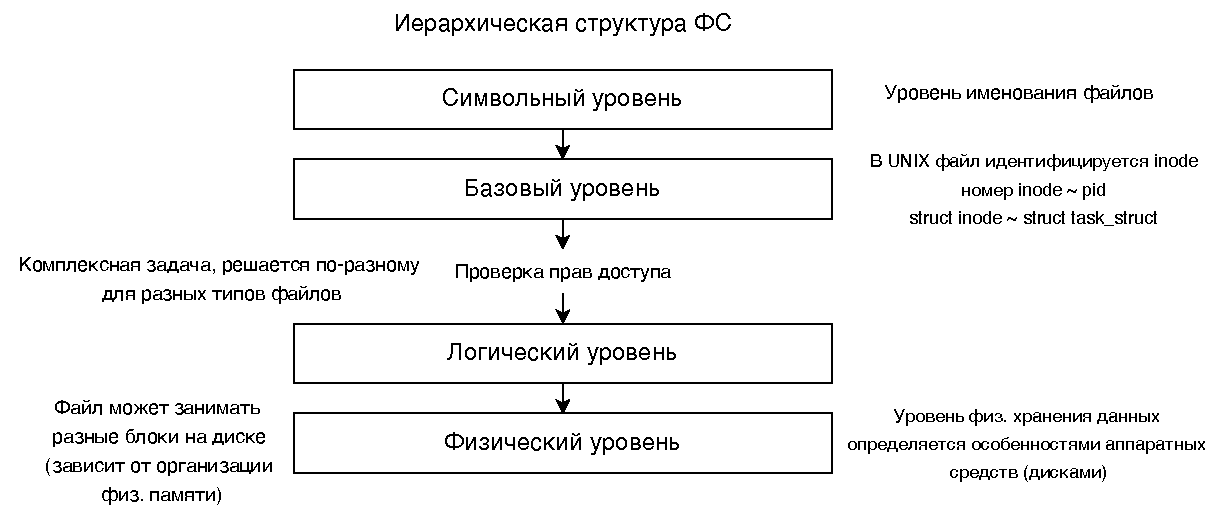
\includegraphics[width=0.8\linewidth]{./images/ierarh_fs.pdf}
  \end{tabular}
\end{table}

\begin{quote}
\textbf{Символьный уровень}

Это уровень именования файлов. Сюда входит организация каталогов, подкаталогов.

В Unix/Linux имя файла не является его идентификатором. Один и тот же файл может иметь множество имён (hard link). Это делалось для того, чтобы к одному и тому же файлу можно было получать доступ из разных директорий. Файлы в системе идентифицируются с помощью inode.

Символьный уровень — самый верхний уровень файловой системы, именно он связан с именованием файлов и позволяет пользователю работать с файлами (так как помнить inode своих файлов сложно).

\textbf{Базовый уровень}


Это уровень формирования дескриптора файлов. Должны быть соответствующие структуры, позволяющие хранить необходимую для файла информацию.

В ядре существует два типа inode (Index Node): дисковый и ядрёный. Чтобы получить доступ к файлу требуется перейти с символьного уровня к номеру inode, которым и идентифицируется в системе файл.

Обоснованием использования двух типов inode в системе является факт того, что Unix изначально создавалась как система которая поддерживает очень большие файлы. Для того чтобы адресовать данные которые находятся в этих файлах, необходимо иметь соответствующие структуры. Так как именно inode как сейчас принято говорить, является дескриптором файла, то такая информация должна храниться в дисковом inode.

\textbf{Логический уровень}

Логическое адресное пространство файла аналогично адресному пространству процесса: оно начинается с нулевого адреса и представляет собой непрерывную последовательность адресов.

\textbf{Физический уровень}

Это уровень хранения и доступа к данным.

\end{quote}

\section{Виртуальная файловая система VFS в Linux}

Файловая система Linux.

Отличается от файловой системы UNIX предоставляемым интерфейсом: ОС Unix и Linux позволяют работать с большим количеством файловых систем.

Для этого UNIX предоставляет интерфейс VFS/vnode, а в Linux — VFS (отказались от vnode).

\begin{table}[h!]
  \centering
  \begin{tabular}{p{1\linewidth}}
    \centering
    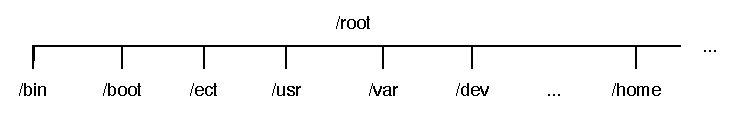
\includegraphics[width=0.8\linewidth]{./images/root.pdf}
  \end{tabular}
\end{table}

«Родные» файловые системы для Linux — ext (ext2, ext4, ...).

Структура слоев VFS:

\begin{table}[h!]
  \centering
  \begin{tabular}{p{1\linewidth}}
    \centering
    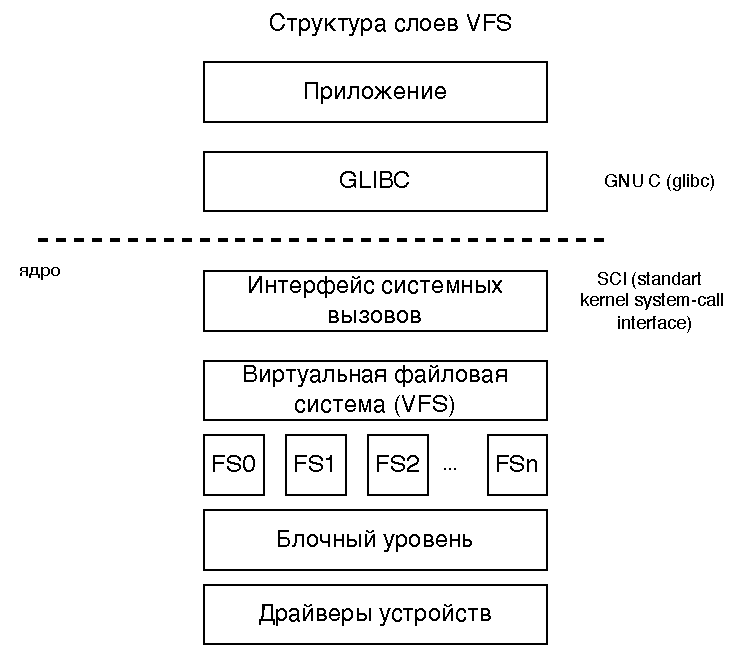
\includegraphics[width=0.8\linewidth]{./images/VFS_struct.pdf}
  \end{tabular}
\end{table}

\section{Четыре структуры VFS – super\_block, inode, dentry, file их назначение}

Внутренняя организация VFS базируется на 4 структурах.

\begin{itemize}
    \item super\_block;
    \item dentry;
    \item inode;
    \item file.
\end{itemize}

\subsection{Связи структур}
Связь структур VFS на основе полей структур --- ключ к работе системы.

Одной из отправных точек являются системные вызовы, связанные с файлами: read/write/lseek. 

Эти системные вызовы работают только с открытыми файлами: чтобы работать с файлом, его нужно открыть.

\textbf{Упрощенная схема}
\begin{table}[h!]
  \centering
  \begin{tabular}{p{1\linewidth}}
    \centering
    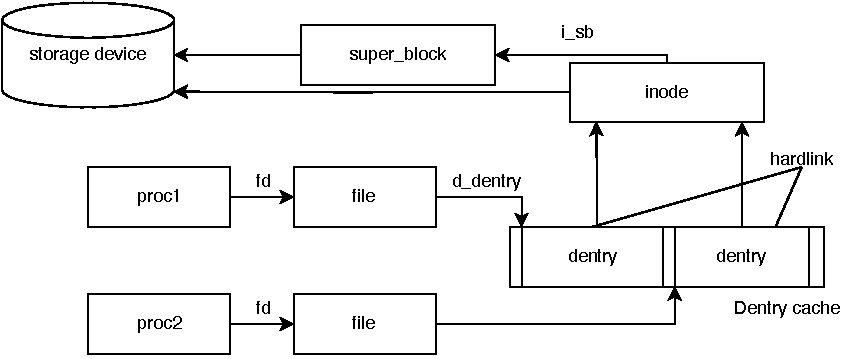
\includegraphics[width=0.8\linewidth]{./images/struct_connect.pdf}
  \end{tabular}
\end{table}

Обычные файлы --- регулярные. inode должен содержать информацию об адресах блоков диска, в которых хранится информация, записываемая в файл. Поэтому суперблок должен содержать соответствующую информацию о блоках на диске (свободен/занят), об inode'ах, иметь ссылку на соответствующую таблицу инодов.

\textbf{Связи структур при выполнении системных вызовов}
\begin{table}[h!]
  \centering
  \begin{tabular}{p{1\linewidth}}
    \centering
    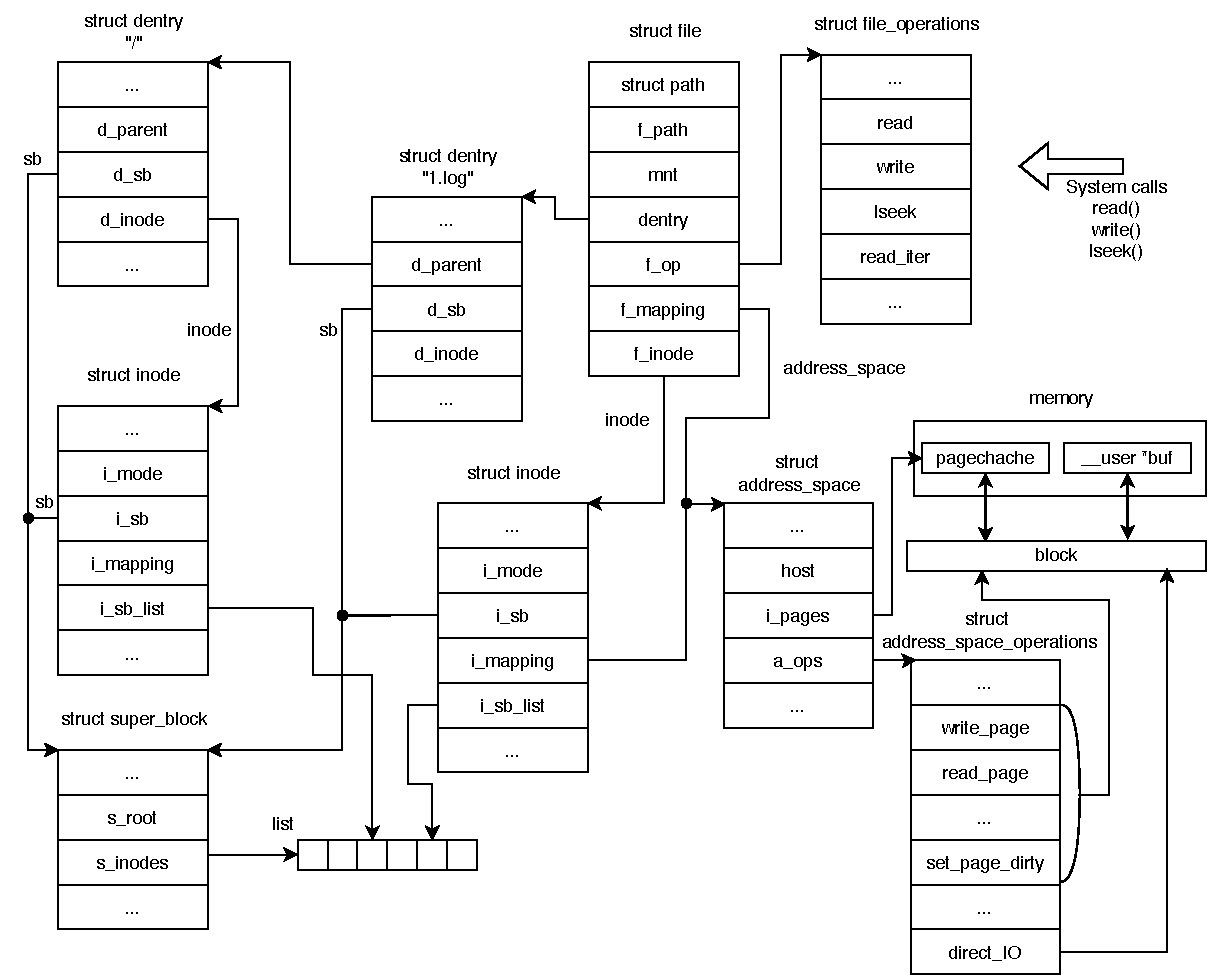
\includegraphics[width=0.8\linewidth]{./images/systemcalls_connect.pdf}
  \end{tabular}
\end{table}

\newpage

\textit{Связь между struct file и struct file operations}

Файл должен быть открыт. Соответственно для открытого файла должен быть создан дескриптор. В этом дескрипторе имеется указатель на struct file\_operations. Это либо стандартные (установленные по умолчанию) операции на файлах для конкретной файловой системы, либо зарегистрированные разработчиком (собственные функции работы с файлами собственной файловой системы).

\textit{Воспоминания о пояснениях}

Указатель f\_mapping показывает связь структур, описывающих файлы в системе с памятью. Также в struct inode есть поле i\_mapping.

struct super\_block содержит список inode (s\_inodes). struct inode содержит указатель на соответствующий inode в списке (i\_sb\_list).

Любая файловая система имеет корневой каталог, а именно от корневого каталога формируется путь к файлу для конкретной файловой системы.

Отправная точка — системные вызовы (read, write, lseek, ...). Здесь нет open(), так как он открывает файл, а использование функций read, write, lseek возможно только при работе с открытым файлом.

\textbf{Связи структур относительно процесса}
\par Теперь пойдем от процесса: Отправная точка -- \textbf{struct task\_struct};
В \textbf{struct task\_struct} есть 2 указателя: 
\begin{itemize}
\item на \textbf{struct fs\_struct} (*fs); - Любой процесс относится к какой-то файловой системе
\item на \textbf{struct files\_struct} (*files) -- дескриптор, описывающий файлы, открытые процессом (Любой процесс имеет собственную таблицу открытых файлов).
\end{itemize}

\begin{table}[H]
  \centering
  \begin{tabular}{p{1\linewidth}}
    \centering
    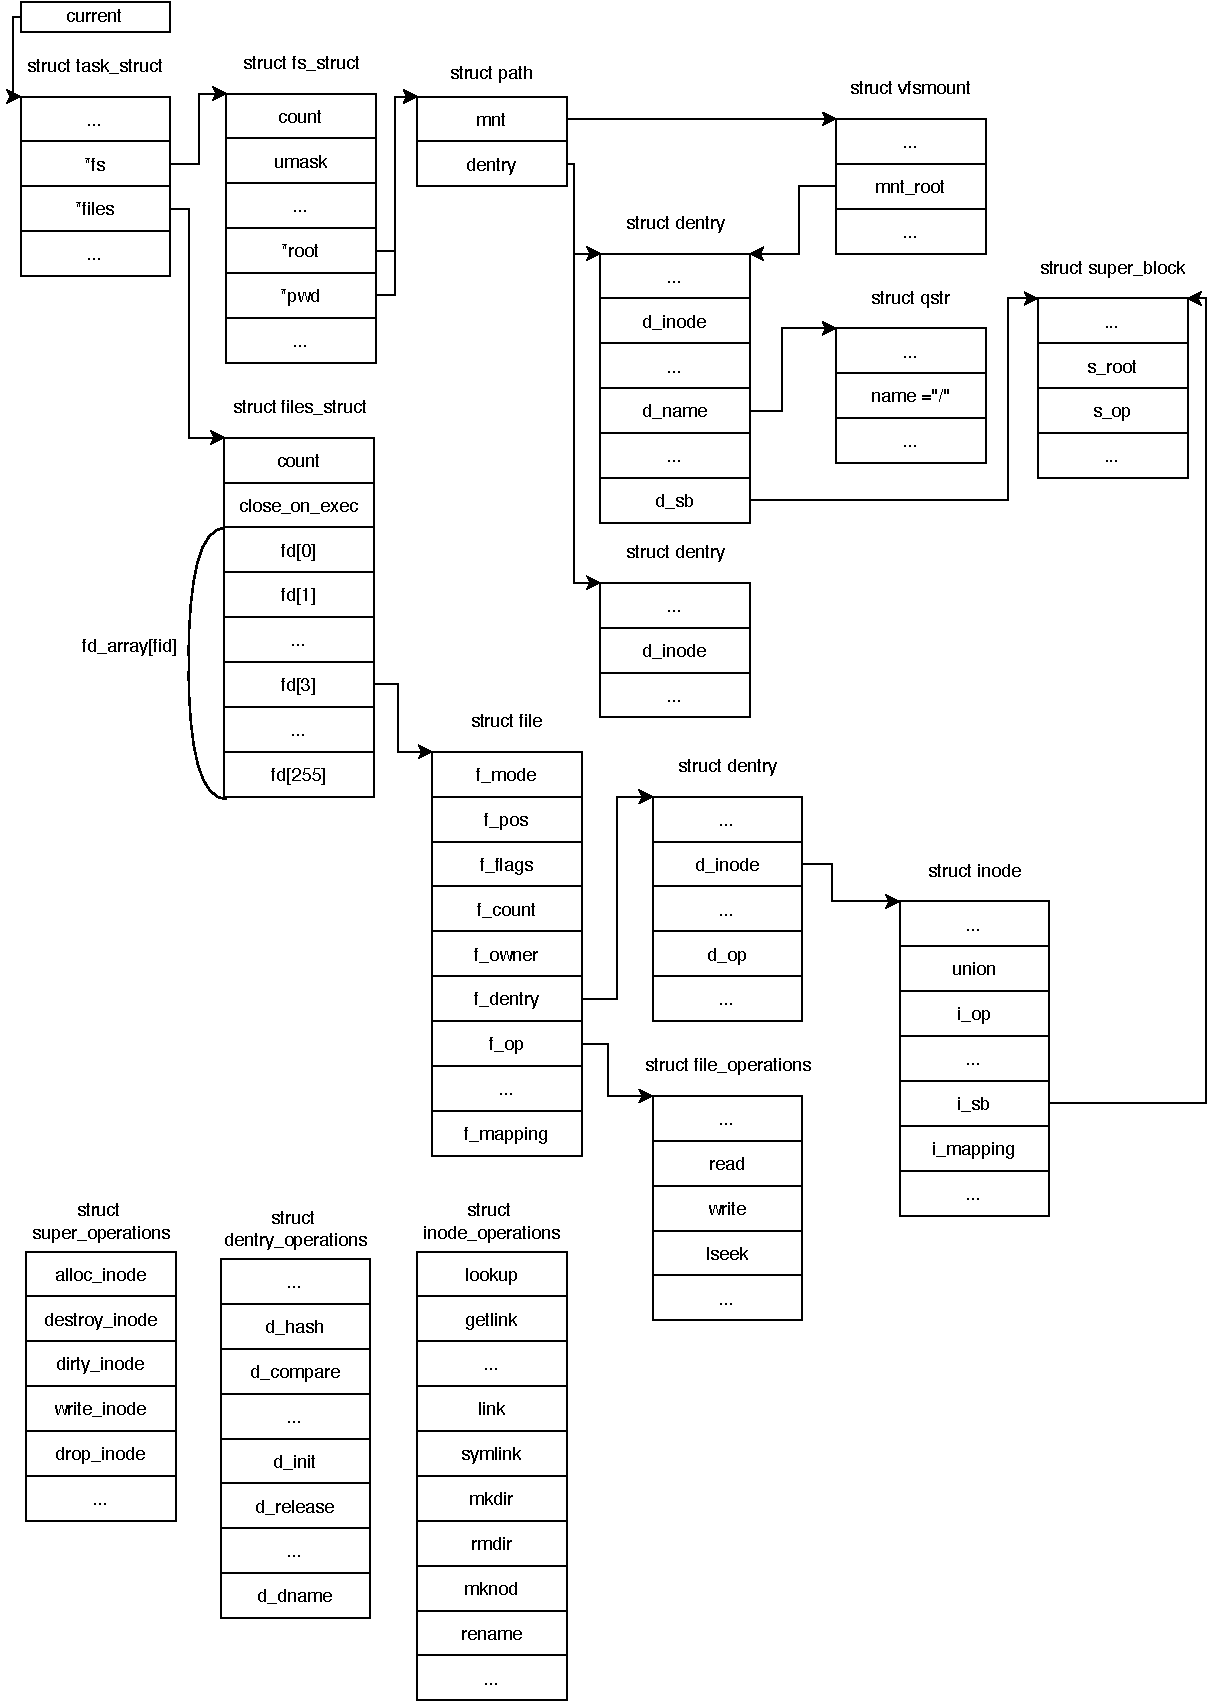
\includegraphics[width=0.8\linewidth]{./images/struct_connect_proc.pdf}
  \end{tabular}
\end{table}

\textit{Воспоминания о зарождении процесса}

\par Каждый процесс до того, как он был запущен, был файлом и принадлежал некоторой \textit{вайбовой} системе, поэтому в \textbf{struct task\_struct} имеется указатель на фс, которой принадлежит файл программы, и указатель на таблицу открытых файлов процесса.
\par Очевидно, что \textbf{struct files\_struct} содержит массив дескрипторов открытых файлов (0,1,2,3,4,...).
\par При этом 
\begin{itemize}
\item 0 -- stdin
\item 1 -- stdout
\item 02-- stderr
\item 03 -- скорая помощь
\end{itemize}
\par Эти файлы открываются для процесса автоматически (файловые дескрипторы для этих файлов создаются автоматически).
\par Когда мы открываем файл, он может получить дескриптор, после этих трех (например, 3,4,5 и тд)
\par Всего в этой таблице может быть 256 дескрипторов.
\par \textbf{struct vfs\_mount} заполняется, когда файловая система монтируется. Имя -- указатель на \textbf{struct qstr}.
\par В \textbf{struct super\_block} есть указатель на \textbf{struct super\_operations} (s\_op) и на root (s\_root), так как корневой каталог (точка монтирования) должен быть создан, чтобы иметь возможность смонтировать файловую систему.

\textbf{Связи структур из лабы на буферы}

\textit{1 open, 2 fdopen, буферизация, читали 20 и 6 байт, выводили на экран}
\begin{table}[H]
  \centering
  \begin{tabular}{p{1\linewidth}}
    \centering
    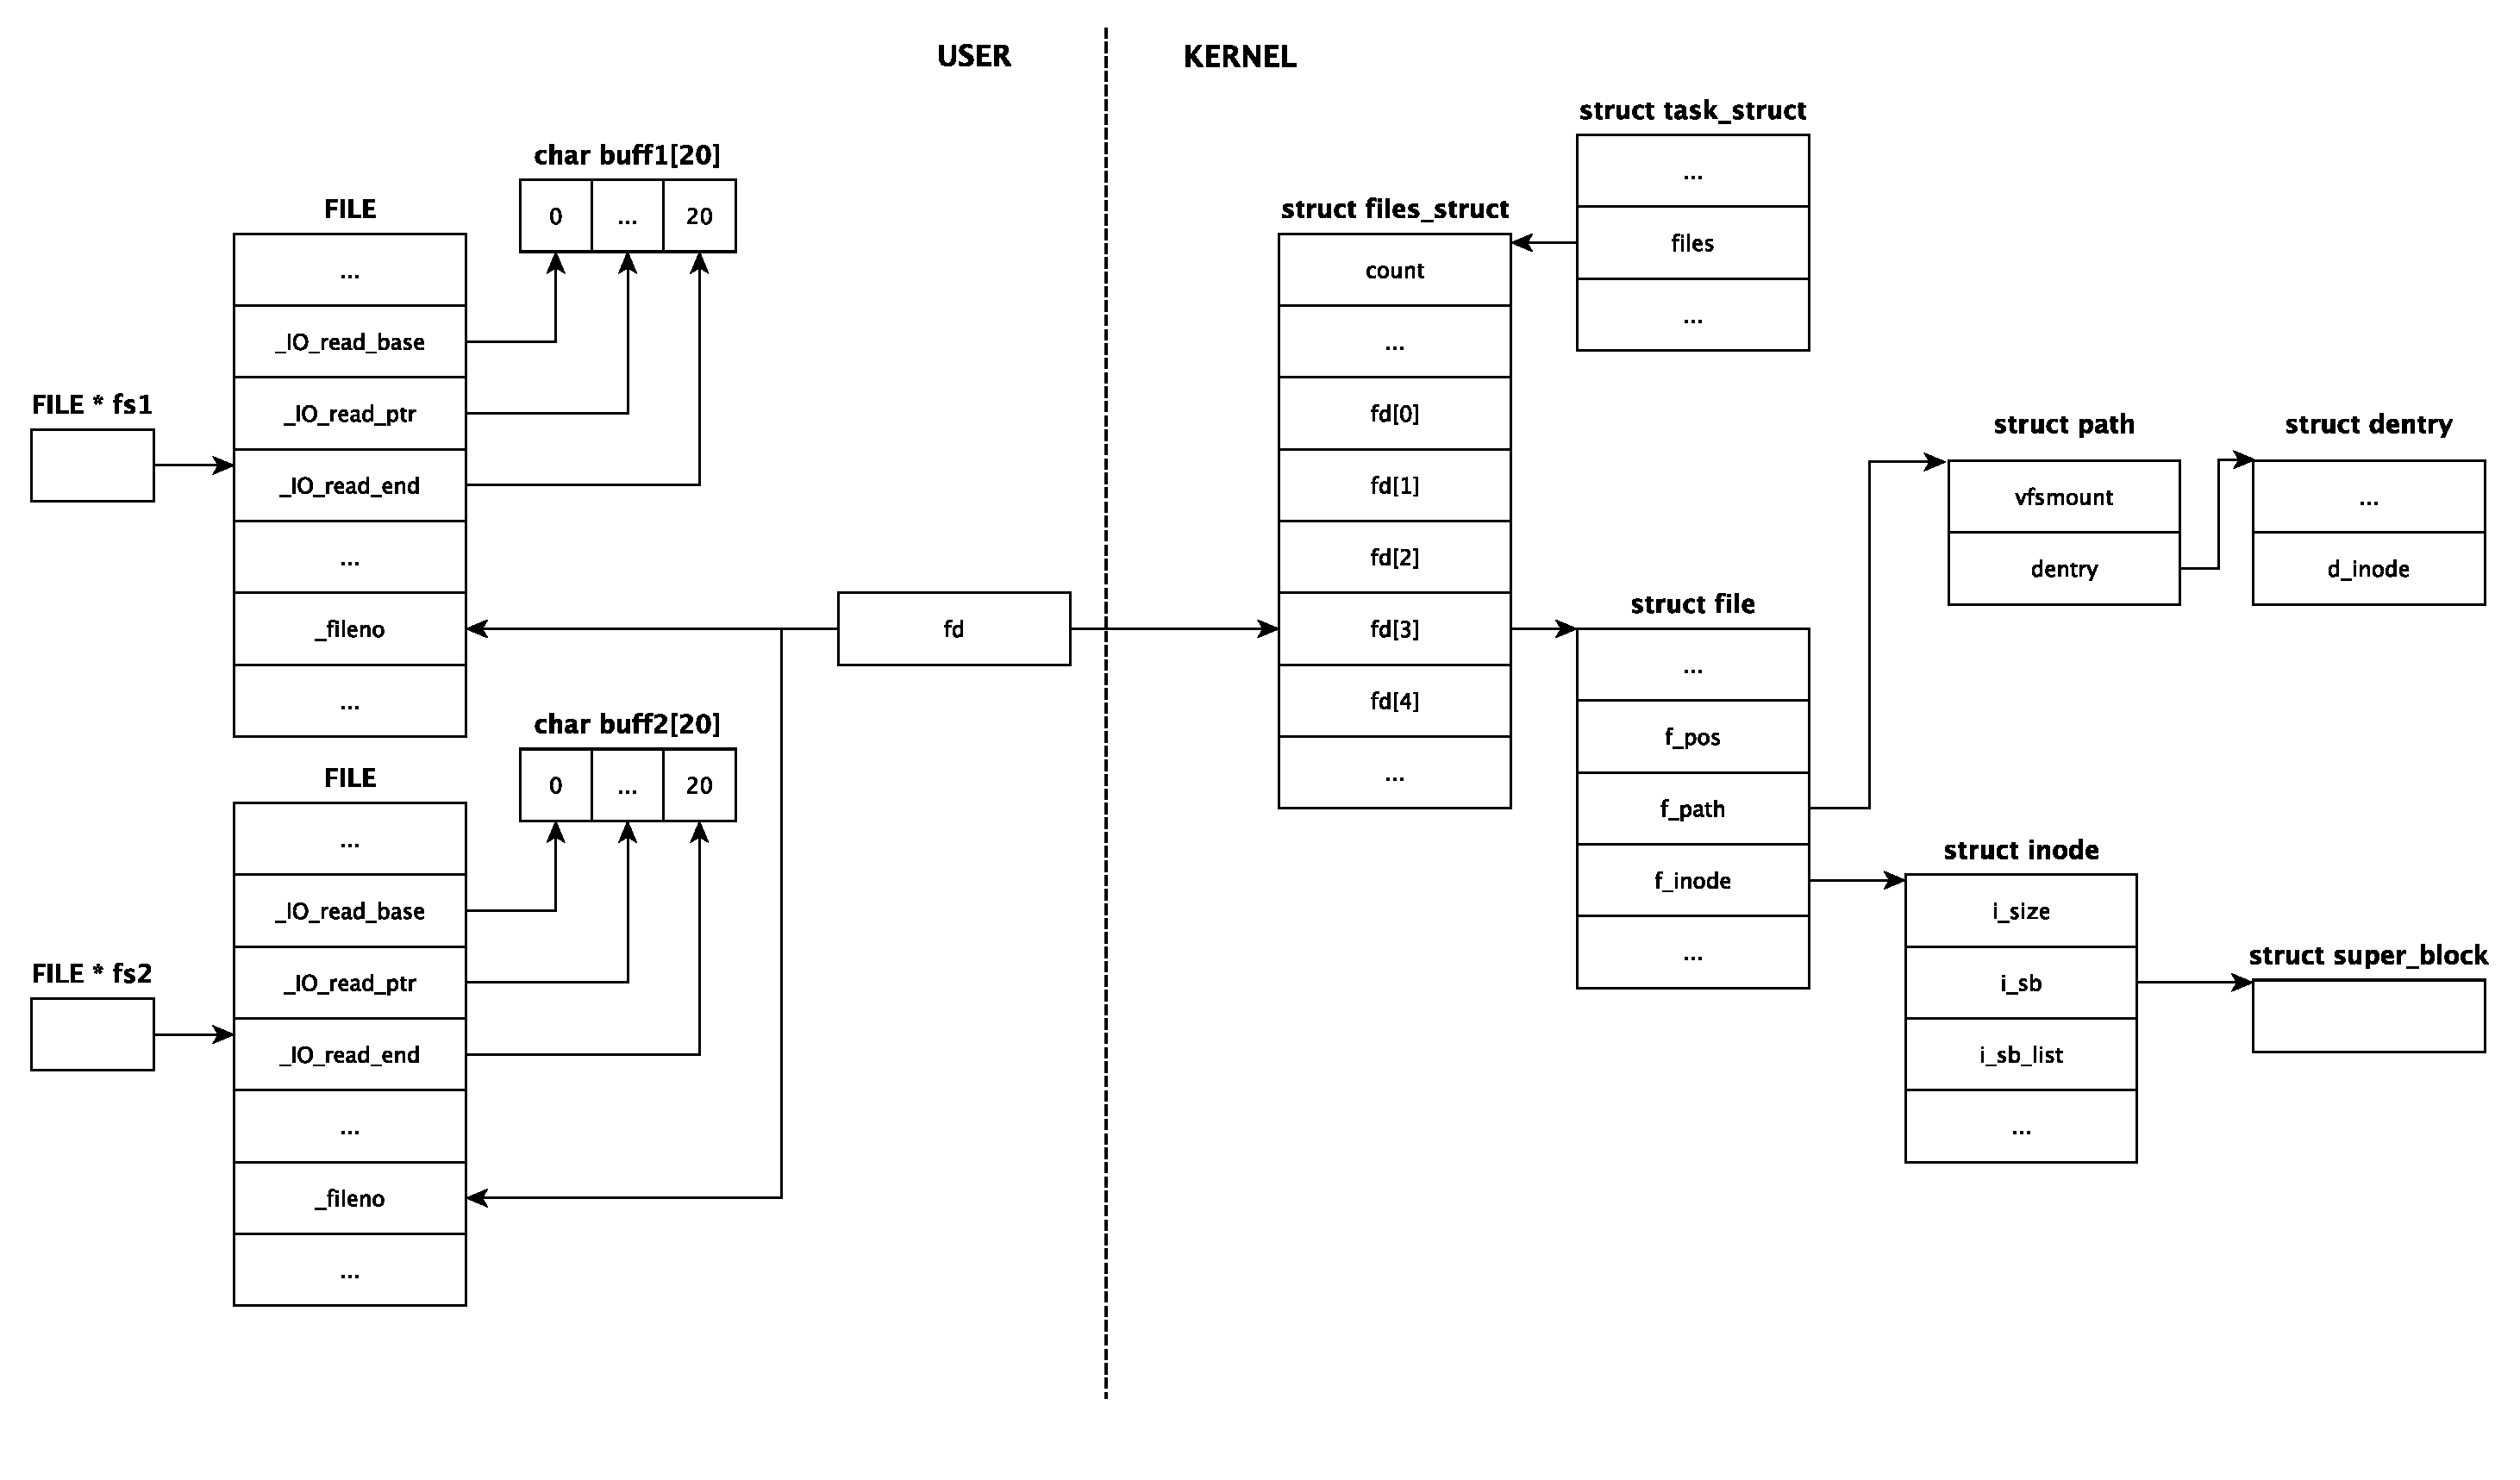
\includegraphics[width=0.8\linewidth]{./images/scheme1.pdf}
  \end{tabular}
\end{table}

\textit{2 open, 2 дескриптора, без буферизации, посимвольно читали и выводили}
\begin{table}[H]
  \centering
  \begin{tabular}{p{1\linewidth}}
    \centering
    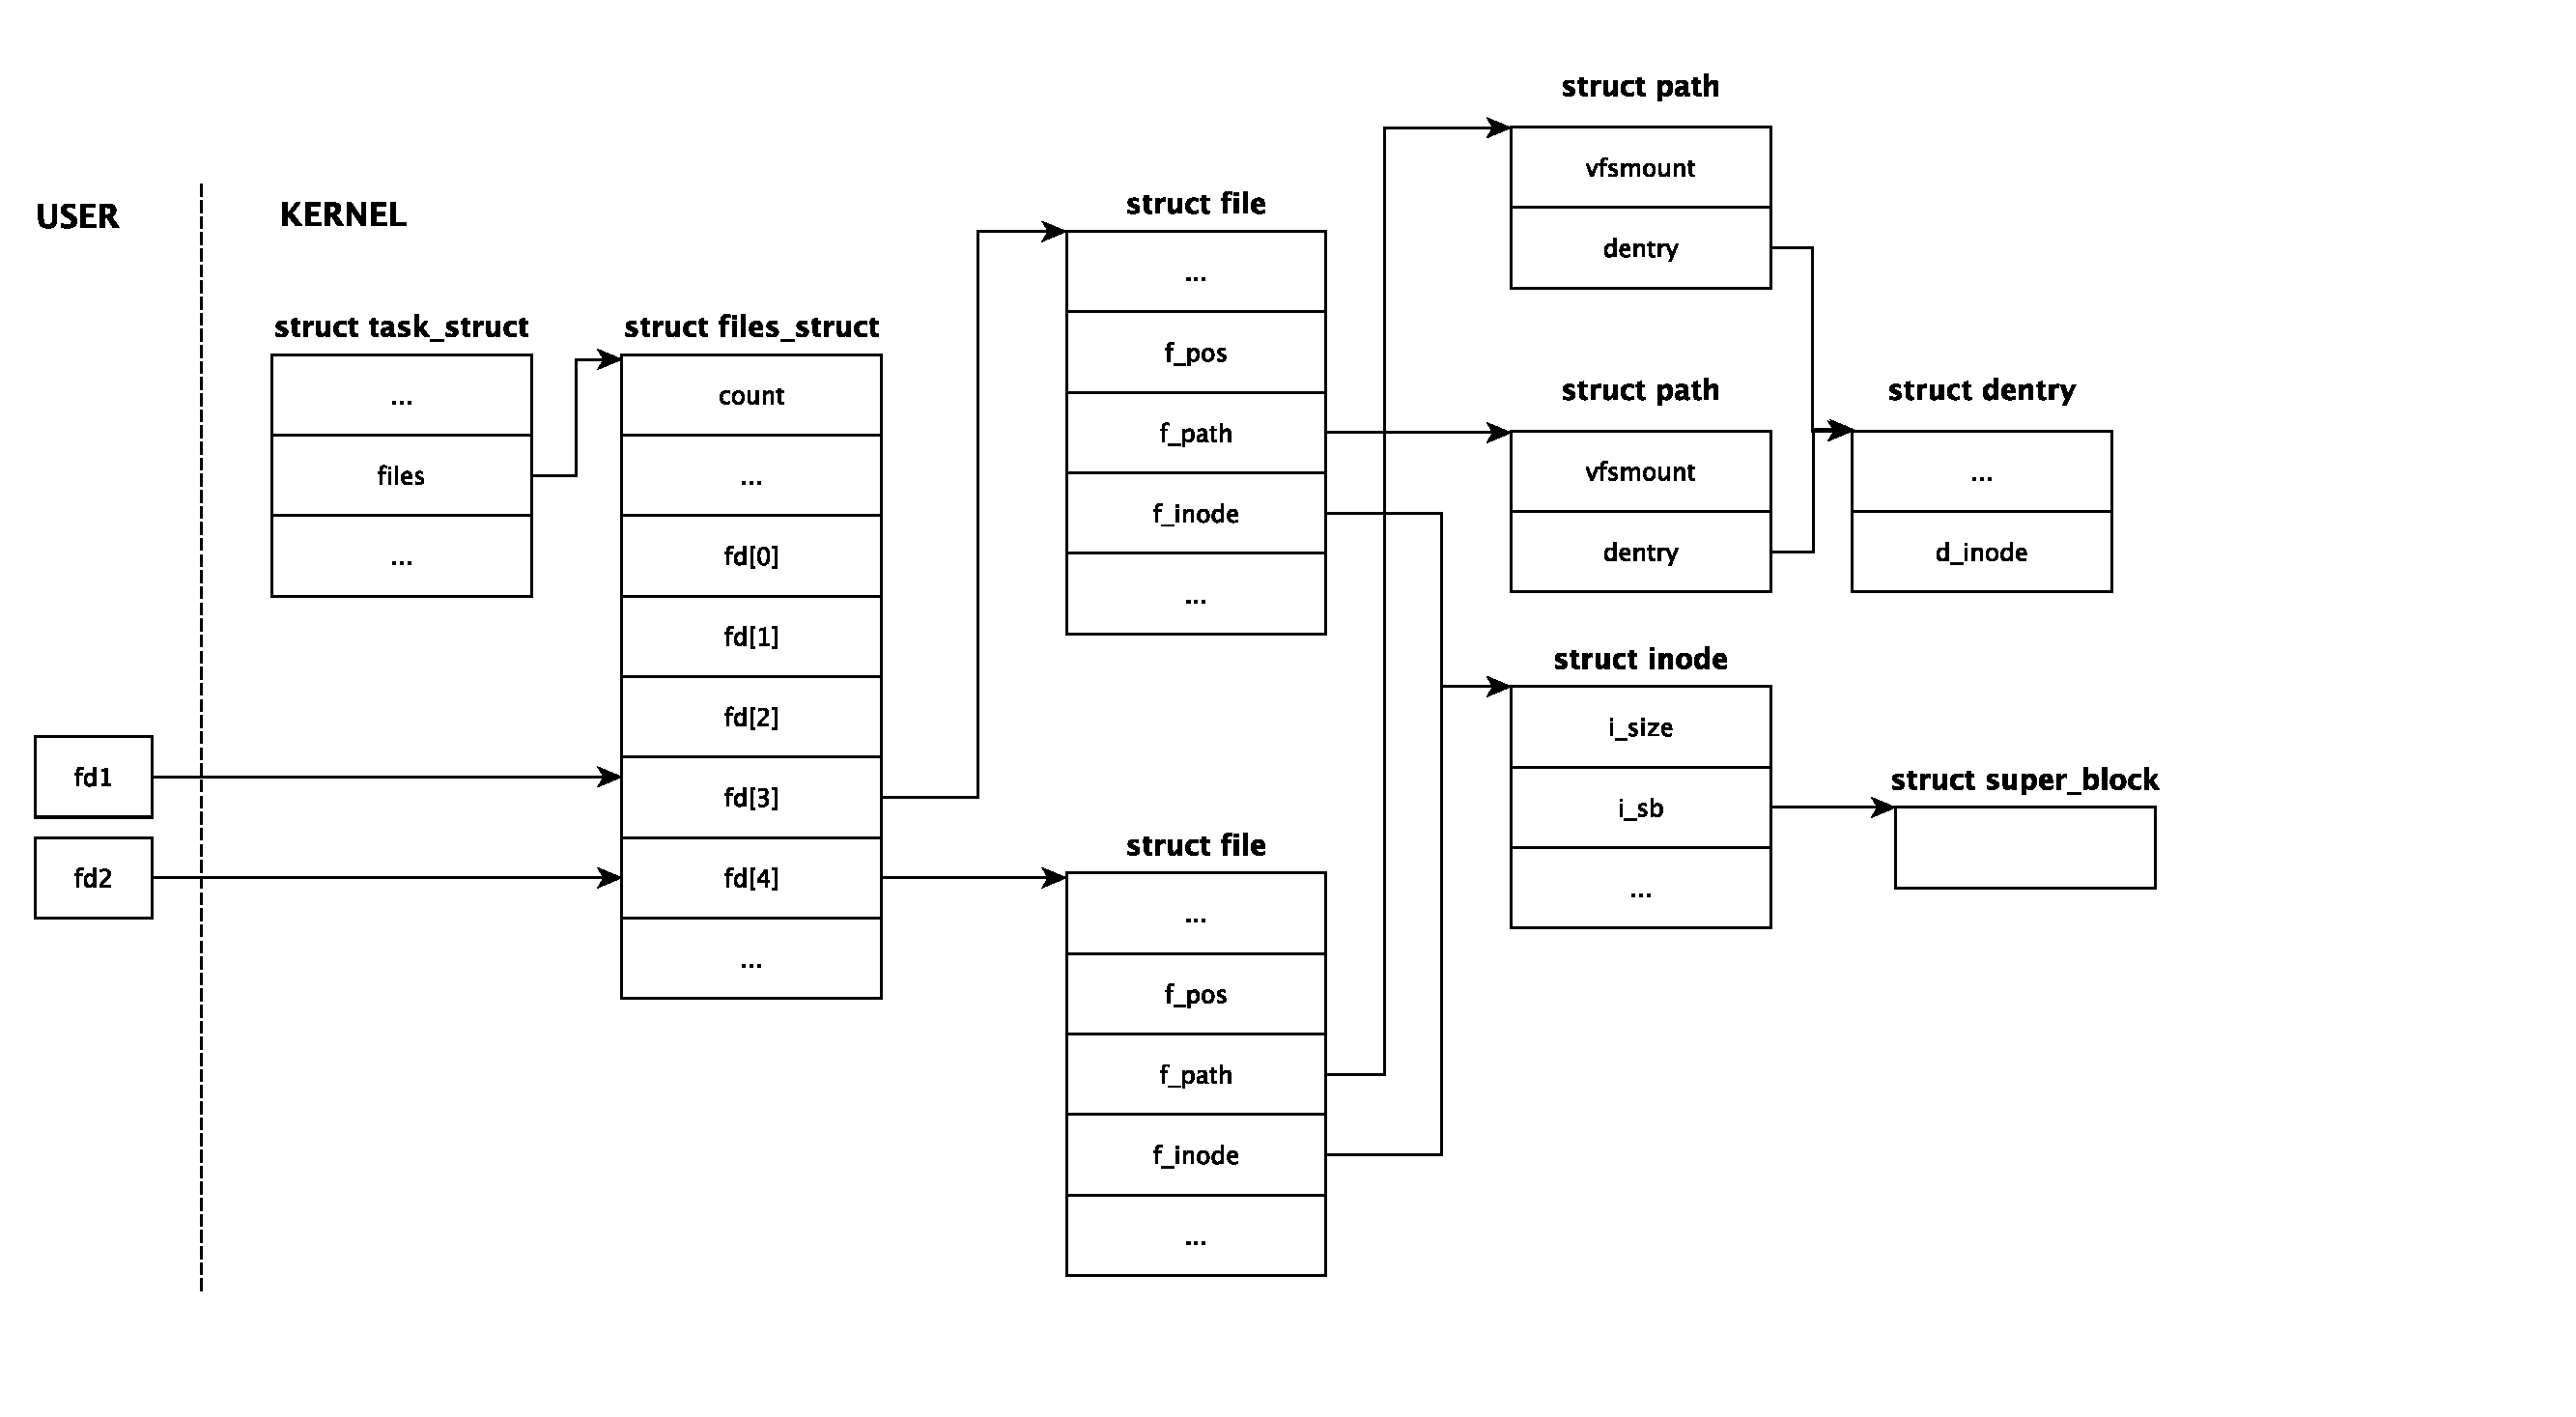
\includegraphics[width=0.8\linewidth]{./images/scheme2.pdf}
  \end{tabular}
\end{table}

\textit{2 open, без буферизации и с ней, шли от а до з писали по очереди, 2 разных дескриптора, свои фпоз, записался либо по последнему фклоуз (при буф), либо по райт (посимвольно затирается без буф)}
\begin{table}[H]
  \centering
  \begin{tabular}{p{1\linewidth}}
    \centering
    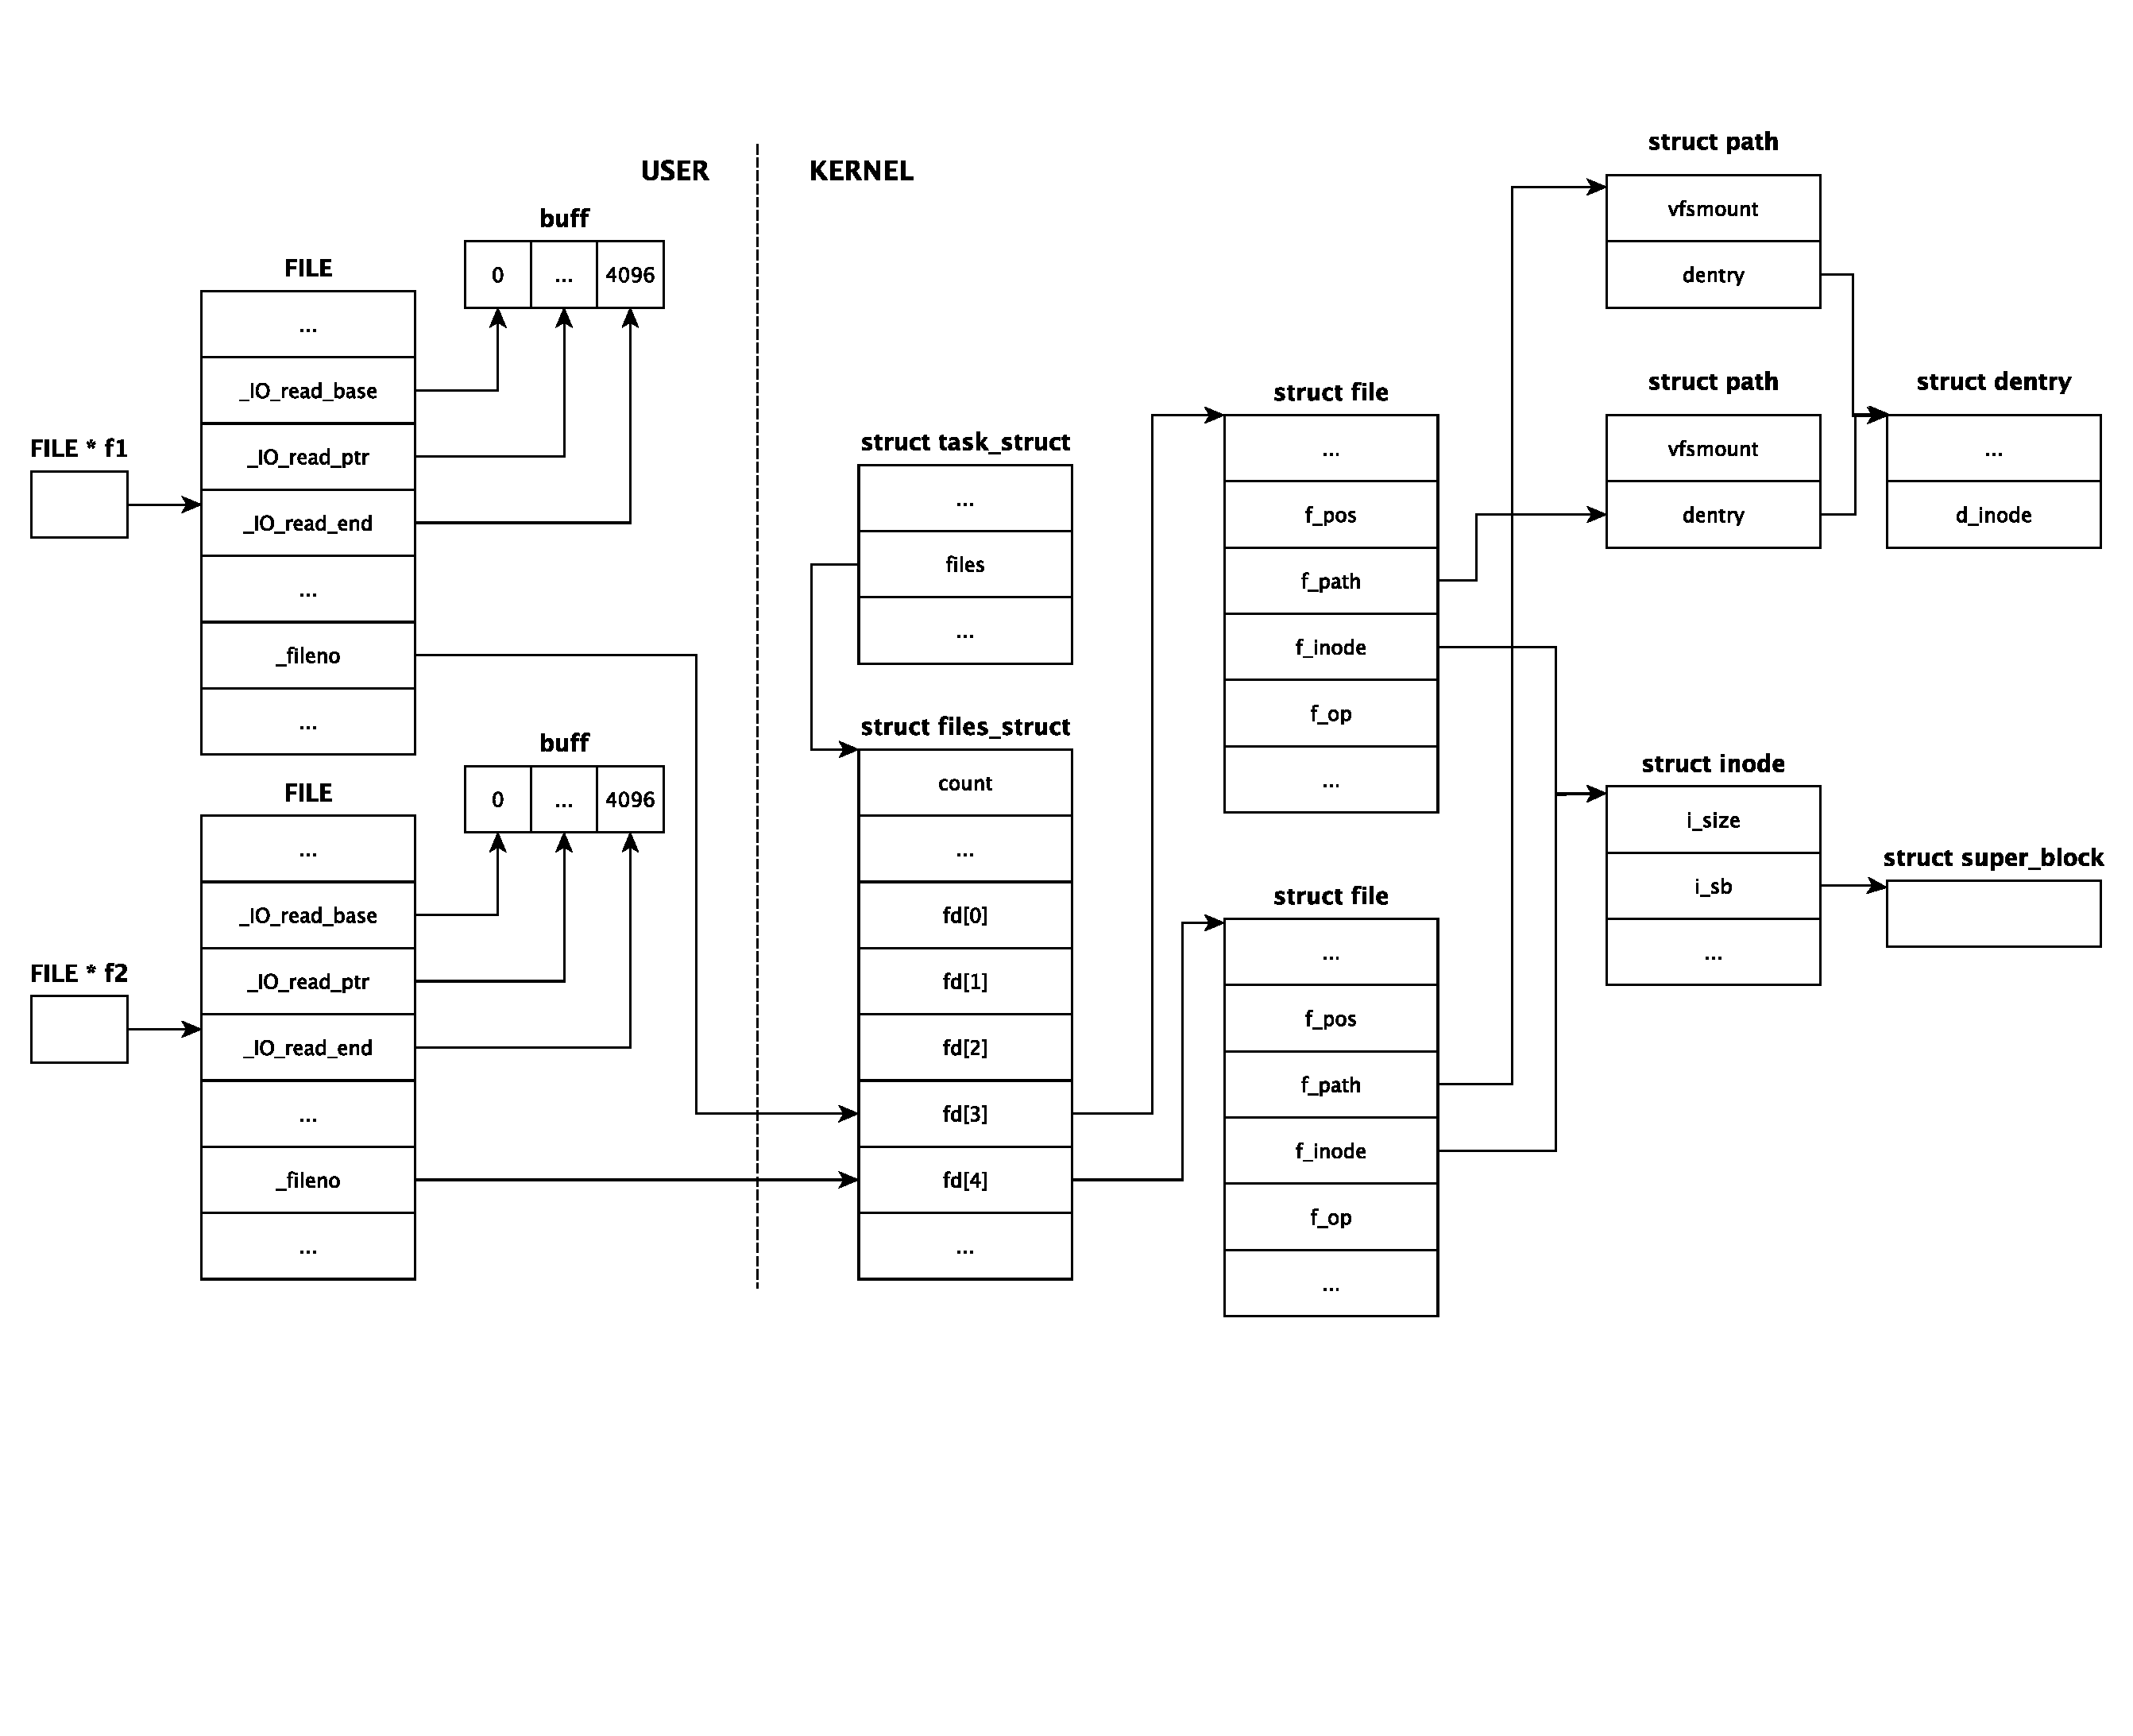
\includegraphics[width=0.8\linewidth]{./images/scheme3.pdf}
  \end{tabular}
\end{table}


\subsection{struct super\_block}

struct super\_block описывает подмонтированную файловую систему на диске.

Именно он обеспечивает возможность работы с файловой системой.

Содержит информацию для обеспечения доступа к файлам, которые хранятся на дисках вразброс, то есть адресацию соответствующих участков диска.

В struct super\_block содержится информация, необходимая системе для управления подмонтированной файловой системой.

У каждой файловой системы может быть один super\_block.

\textbf{Определение struct super\_block}

\begin{lstlisting}
struct super_block {
        struct list_head        s_list;            
        dev_t                   s_dev;            // устройство, на котором находится ФС
        unsigned long           s_blocksize;       // размер блока в байтах
        unsigned char           s_dirt;           // флаг изменения супрблока
        struct file_system_type s_type;            // в ядре есть структура описывающая тип ФС
        struct super_operations s_op;             // операции на суперблоке
        struct block_device *b_dev // описывает устройство, на котором находится файловая система (соответствует драйверу блочного устройства)
        unsigned long            s_magic;         // магический номер смонтированной ФС
        struct dentry            *s_root;      //  точка монтирования ФС
        ...
        int                      s_count;       // число ссылок
        struct list_head         s_dirty;         // список измененных inode'ов
        char                     s_id[32];      // имя?
};
\end{lstlisting}

\textbf{Определение struct super\_operations}

На любой структуре, описывающей объект ядра, определены функции для работы с объектом соответствующего типа (struct file\_operations, struct inode\_operations, struct dentry\_operations).

\begin{lstlisting}
<linux/fs.h>

struct super_operations
{
  struct inode *(alloc_inode)(struct superblock *sb);
void (*destroy_inode) (struct inode *);
...
void (*dirty_inode)(struct inode *, int flags);
int (*write_inode)(struct inode*, struct wirteback_cintrol *wbc);
int (*drop_inode)(struct inode *);
...
void (*put_super)(struct super_block *);
}

\end{lstlisting}


dirty\_inode вызывается VFS, когда в индекс (inode) вносятся изменения (функция используется для изменения соответствующей табилцы структуры).

Ядро хранит копию таблицы inode'ов в памяти ядра (так как доступ к диску — медленная операция), то есть inode, к которым были обращения, кешируются для ускорения доступа к файлам.

Сначала изменения вносятся в таблицу, которая находится в оперативной памяти.

Функция dirty\_inode позволяет отметить, что inode был изменен, и эту информацию надо скопировать в таблицу, которая находится на диске.

write\_inode предназначена для записи inode на диск и помечает inode как измененный.

put\_super вызывается VFS при размонтировании ФС.

\textbf{Подробное описание}

Основная информация, которую хранит super\_block — информация, которая обеспечивает доступ к таблице inode'ов, и каждый дескриптор inode обеспечивает информацию для доступа к данным, хранящимся в файле. В struct super\_operations есть функция alloc\_inode (принимает super\_block, так как любой файл должен принадлежать конкретной файловой системе, то есть конкретному суперблоку; конкретный суперблок обеспечивает доступ к конкретному файлу).

Функция alloc\_super создает новый superblock. Вызывается при монтировании файловой системы. Возвращает указатель на новый superblock или NULL, если не удалось выделить superblock.

\begin{quote}

Функция alloc\_super создает новый superblock:

\begin{lstlisting}
static struct super_block *alloc_super (
  struct file_system_type *type,
  int flags,
  struct user_namespace *user_ns
)
{
  struct superblock *s = kzalloc(sizeof(struct super_block), GFP_USER);
  static const struct super_operations default_ops;
  if (!s) return NULL;
  INIT_LIST_HEAD(&s->s_mounts);
  ...
  INIT_LIST_HEAD(&s->s_inodes);
  ...
}
\end{lstlisting}

default\_ops: Для любой файловой системы определяется набор операций на суперблоке (система предоставляет разработчику определить эти операции).

s\_mounts: Одна и та же файловая система может быть смонтирована много раз, при этом она будет иметь один тип.

Любой экземпляр (объект) super\_block описывает конкретную файловую систему, которая может быть подмонтирована, и только тогда файлы этой файловой системы будут доступны пользователю.
\end{quote}

\subsection{struct dentry}

struct dentry (directory entry) описывает экземпляр директории, нигде не хранится, создается на основе информации, которая хранится в директориях на диске (inode с диска).

\sout{struct dentry не имеет mapping, то есть нигде не отображена.}

\sout{Именно поэтому} имена поддиректорий хранятся как обычные файлы, так как эта информация нужна системе, чтобы предоставить в распоряжение пользователя имена директорий и поддиректорий.

\sout{Дерева каталогов не существуют, то есть оно строится "на лету" (например, утилитой tree) на основе той информации, которая сохранена на диске.} Чтобы ускорить обращение к этой информации, она вся кешируется.

То есть когда происходит первое обращение к каталогу, он кешируется (существует соответствующая struct list\_head, в которой будет хранится информация об этом каталоге).

struct dentry описывает элемент пути. Элемент пути — часть пути к файлу, которые отделяются друг от друга «/», начиная с корневого каталога.

Про объекты dentry:
\begin{itemize}
\item  информация о любом элементе пути хранится как файл.
\item существует кеш объектов dentry, в котором хранятся элементы пути, к которым уже были обращения. Это ускоряет доступ к файлам.
\end{itemize}

\begin{quote}
Объект dentry может находиться в одном из 4 состояний:
\begin{enumerate}
\item free

Не содержит достоверной информации и не используется VFS. Соответствующая область памяти обрабатывается SLAB allocator'ом.
\item unused

В настоящее время ядром не используется. Счетчик d\_count равен нулю, но поле d\_inode по-прежнему указывает на соответствующий индексный дескриптор. Неиспользуемый объект dentry содержит достоверную информацию, но при необходимости он может быть удален и память может быть освобождена.

\item in use

Используется ядром в текущий момент. Счетчик d\_count больше нуля. У такого объекта есть inode (поле d\_inode указывается на соответствующий дескриптор). Такой объект dentry не может быть удален.

\item negative

Для него не существует соответствующий ему inode. Это возможно, если соответствующий inode был удален с диска или объект dentry был создан как элемент пути несуществующему файлу.

Поле d\_inode = NULL, но объект все еще находится в кеше dentry.

Объекты dentry in use могут стать negative, если удаляется последний hard link на соответствующий файл. В этом случае объект dentry перемещается в список LRU unused\_dentry.
\end{enumerate}
\end{quote}

\textbf{Определение struct dentry}

\begin{table}[H]
\begin{tabular}{|l|l|l|}
\hline
type                        & field         & description                                                                                                                                                                                                                                                                                                                                  \\ \hline
atomic\_t                   & d\_count      & \begin{tabular}[c]{@{}l@{}}Кол-во использований\\ объекта dentry\end{tabular}                                                                                                                                                                                                                                                                \\ \hline
unsigned int                & d\_flags      & \begin{tabular}[c]{@{}l@{}}Флаги, определенные\\ для конкретного \\ объекта dentry\end{tabular}                                                                                                                                                                                                                                              \\ \hline
struct dentry *             & d\_parent     & \begin{tabular}[c]{@{}l@{}}Указатель на\\ родительский каталог\end{tabular}                                                                                                                                                                                                                                                                  \\ \hline
struct list\_head           & d\_hash       & \begin{tabular}[c]{@{}l@{}}Указатель на список\\ в хеш-таблице\\ (указатели на соседние\\ элементы в списке, \\ связанные с одним и тем же\\ значением хеш-функции)\end{tabular}                                                                                                                                                             \\ \hline
\end{tabular}
\end{table}

\begin{table}[H]
\begin{tabular}{|l|l|l|}
\hline
type                        & field         & description                                                                                                                                                                                                                                                                                                                                  \\ \hline
struct list\_head           & d\_lru        & \begin{tabular}[c]{@{}l@{}}Указатель на список dentry\\ в состоянии unused\\ (очищается по алгоритму\\ LRU, то есть вытесняются\\ dentry, к которым дольше\\ всего не было обращений)\\ (организован по алгоритму\\ LRU, так как какое-то время\\ неиспользуемые dentry\\ хранятся в списке для \\ скорения обращения к файлам)\end{tabular} \\ \hline
struct list\_head           & d\_child      & Список подкаталогов                                                                                                                                                                                                                                                                                                                          \\ \hline
...                         & ...           & ...                                                                                                                                                                                                                                                                                                                                          \\ \hline
int                         & d\_mounted    & \begin{tabular}[c]{@{}l@{}}Флаг, который установлен \textless{}=\textgreater \\ dentry является точкой\\ монтирования ФС\end{tabular}                                                                                                                                                                                                        \\ \hline
struct qstr                 & d\_name       & Имя файла                                                                                                                                                                                                                                                                                                                                    \\ \hline
struct dentry\_operations * & d\_op         & \begin{tabular}[c]{@{}l@{}}Функции (системные вызовы)\\ для работы с dentry\end{tabular}                                                                                                                                                                                                                                                     \\ \hline
struct super\_block *       & d\_sb         & \begin{tabular}[c]{@{}l@{}}Любая директория\\ относится к конкретной\\ файловой системе, то есть\\ дерево каталогов - дерево\\ конкретной файловой системы\\ =\textgreater объект dentry (как эл-т пути)\\ всегда принадлежит конкретной\\ файловой системе\end{tabular}                                                                     \\ \hline
unsigned long               & d\_vfs\_flags & Флаги кеша dentry                                                                                                                                                                                                                                                                                                                            \\ \hline
struct list\_head           & d\_alias      & list of associated inodes                                                                                                                                                                                                                                                                                                                    \\ \hline
\end{tabular}
\end{table}

\textbf{Определение struct dentry\_operations}

\begin{lstlisting}
struct dentry_operations
{
  int (*drevalidate)(struct dentry *, unsigned int);
  ...
  int (*d_hash)(const struct dentry *, unsigned int);
  int (* d_compare)(const struct dentry *, unsigned int, const char *, const struct
  qstr *);
  int (* d_delete)(const struct dentry *);
  int (* d_init)(const struct dentry *);
  int (* d_release) (struct dentry *);
  void (* d_input)(struct dentry *, struct inode *);
  char *(* d_name)(struct dentry *, char *, int);
  ..
}
\end{lstlisting}

Краткое пояснение полей структуры:
\begin{itemize}
\item d\_hash — хеширование;
\item d\_compare — сравнение: когда мы проходим по пути к файлу, мы сравниваем заданное имя и найденное.
\item d\_init — выделение dentry.
\item d\_release — освобождение dentry: освободить dentry можно, если на него нет ссылок;
\item d\_dname — определение/создание пути к эл-ту (объекту) dentry.
\end{itemize}

Подробное пояснение полей структуры:
\begin{itemize}
\item d\_hash — вызывается, когда VFS добавляет dentry в хеш-таблицу.

Первый dentry, который добавлен с помощью d\_hash, является родительским каталогом.
\item d\_compare — вызывается для того, чтобы сравнить заданное имя с именем dentry; При этом первый dentry является родителем того dentry, который сравнивается.

В параметрах const struct qstr * — имя, с которым надо сравнить.
\item d\_delete вызывается, если удаляется последующая ссылка на dentry.
\item d\_init вызывается при создании.
\item d\_releae вызывается при освобождении.
\item d\_input вызвается, когда dentry теряет inode.
\item d\_name вызывается, когда необходимо сгенерировать путь к элементу dentry.
\end{itemize}

\textbf{Кеш dentry}

\begin{quote}
in english: dentry\_cache

Обращение к диску — очень длительная операция. 

Информация об элементе пути (dentry) имеет inode (хранится на диске в виду файла).

Таких элементов пути к файлу может быть много, так как папки можно вкладывать одну в другую. Каждое вложение — дополнительный объект dentry (элемент пути), то есть файл.

При обращении к файлу просматриваются все элементы пути (каждый раз — обращение к диску, поэтому объекты dentry хранятся в кеше, это существенно уменьшает время обращения к конкретному файлу). При этом они не удаляются просто так, так как могут использоваться позже.
\end{quote}

В Linux кеш dentry состоит из 2 типов структур./
\begin{enumerate}
\item set of dentry object в следующих состояниях: in use, unuse, negative.
\item hash table для быстрого получения объекта dentry, который связан с заданным именем файла и заданным каталогом.
\end{enumerate}

Если объект, к которому происходит обращение, не включен в кеш dentry, то функция хеширования возвращает нулевое значение.

Кеш dentry фактически действует как контроллер для cache inode. То есть кроме кеша dentry есть cache inode (slab cache - его часть).

Все эти кеши хранятся в оперативной памяти.

Все неиспользуемые данные включены в двусвязный список, который обновляется по алгоритму LRU.

Адреса первого и последнего элемента списка LRU хранятся соответственно в полях next и prev переменной dentry\_unused.

\begin{quote}
Воспоминания о списках в ядре.

В ядре используются двусвязные списки для обеспечения быстрого доступа за счет реализации соответствующих алгоритмов, простейшим из которых является бинарный поиск.
\end{quote}

Каждый объект dentry в состоянии in use включается в двусвязный список (поле i\_dentry) соответствующего объекта inode (i\_dentry <- inode).

Поле d\_alias хранит адреса соседних элементов в списке.

\subsection{struct inode}

\textbf{Кратко}

struct inode -- дескриптор физического файла. Существует 2 типа inode.
\begin{enumerate}
    \item Дисковый -- описывает физ. файл.
    \item inode в ядре, к-ый позволяет предварительно контролировать доступ к файлу.
\end{enumerate}

\sout{regular file -> обращается к дисковому inode; pipe, socket и др. спец. файлы должны существовать не в superblock (доступ к ним должен осуществляться не через superblock)}

\textbf{Подробнее}

\sout{Информация в inode ядра актуальна для ядра, для динамического обращения.}

В дисковом inode хранится информация о физ. расположении файла на диске. У struct inode есть номер (inode number) -- индекс (смещение к inode в таблице inode-ов)

В UNIX/LINUX имя файла не явл его идентификатором. Идентификатором файла явл. номер inode.

Физ. файлы, если говорить об обычных файлах хранятся на диске. Чтобы создать файл для него нужно создать inode, а затем для него должно быть выделено адр. пр-во диска.

Обращение к файлу --- обращение к inode.

Иерархическая структура каталогов очень удобна для доступа к файлам.

Доступ к любому элементу каталога осуществляется по его индексу (номеру inode).

На диске должны хранится файлы содержащие информацию о регулярных файлах и файлах-директориях, чтобы  эта информация мб представлена в виде дерева каталогов.

inode содержат информацию и о файлах-директориях, и об обычных файлах (об их расположении на диске).

Команды для получения информации об inode

ls -i --- увидеть inode

df --- увидеть список файловых систем, при этом в списке мы увидим, сколько inode содержит ФС, сколько айнодов используется, сколько свободных айнодов,\% использования айнодов и точку монтирования.

Информацию из айнод файла можно получить в user mode, используя команду stat:

file: user.txt

Size: 78   Blocks: 8     IO Block: 4096

Device 

Access

\subsubsection{определение struct inode}

Но кроме обычных файлов в UNIX/Linux есть прогр. каналы, сокеты, гибкие ссылки и внешние устройтва. Они имеют inode.

struct inode содержит union, в котором перечисляются типы файлов, и union, в котором перечисляются inode соответствующих фс

\begin{lstlisting}
struct inode {
  struct list_head i_hash;
 struct list_head i_list;
 struct list_head i_dentry;
 ...
 unsigned long i_ino;
 atomic_t i_count;
 kdev_t i_rdev;
 umode_t i_mode;
 ...
 loff_t i_size;
 ...
 // информация о времени модификации и доступа к inode
 ...
 // 6 полей, связ с блоками(только для ядра)
 ...
 unsigned int i_blkbits;// битовая карта блока
 unsigned long i_blksize;// размер блоков
 unsigned long i_blocks;// кол-во блоков
 ...
 const struct inode_operations  *i_op; //перечень функций определенных для работы с inode и c открытыми файлами
 const struct file_operations  *i_fop; 
 struct super_block  *i_sb; 
 ...
 struct list_head i_devices;
 struct pipe_inode_info *i_pipe;
 struct block_device *i_bdev;
 struct char_device *i_cdev;
 ...
 unsigned long i_state;
 unsigned int i_flags;
 ...
 union //типы фс
 {
 struct minix_inode_info minix_i;
 struct ext2_inode_info ext2_i;
 ....
 struct ntfs_inode_info ntfs_i;
 struct msdos_inode_info msdos_i;
 ...
 struct nfs_inode_info nfs_i;// сетевая фс
 struct ufs_inode_info ufs_i;
 ...
 struct proc_inode_info proc_i;
 struct socket socket_i;
 ...
 
 }
};
\end{lstlisting}


i\_hash -- Информацию dentry хешируется для ускорения обращения к файлу и его имени (фактически dentry -- часть имени файла).

Как правило, пользователь многократно обращается к одному и тому же файлу. Для этого в ядре имеются соотв. односвязные списки.


i\_sb:  Любой inode принадлежит конкретной ФС. Cлед-но, struct inode должна содержать указатель на superblock.

\subsection{Структура inode\_operations}
Функции, определенные для работы с inode:
\begin{lstlisting}
    struct inode_operations {
  struct dentry * (*lookup) (struct inode *,struct dentry *, unsigned int);
  
  int (*create) (struct inode *,struct dentry *,
           umode_t, bool);

  int (*mkdir) (struct inode *,struct dentry *,
          umode_t);
  
  int (*rename) ( struct inode *, struct dentry *,
      struct inode *, struct dentry *, unsigned int);
  ...
} ;
\end{lstlisting}

Для поиска inode требуется, чтобы VFS вызывала функцию lookup() родительского каталога inode. Этот метод устанавливается конкретной реализацией файловой системы, в которой находится inode. Как только VFS находит требуемый dentry (и, следовательно, inode), можно открывать файл системным вызовом open или получать информацию о файле функцией stat, которая просматривает данные inode и передает часть их в пространство пользователя.


\subsection{Кеш inode}
Задача кеш inode --- ускорение поиска и доступа.

Кеш inode в Linux:
\begin{enumerate}
    \item Глобальный хеш-массив inode\_hash\_table

    В нем каждый inode хешируется по значению указателя на superblock и 32-разрядному номеру inode. Если superblock отсутствует, то inode добавляется к двусвязному списку anon\_hash\_chain. Такие inode называют \textit{анонимными}. Например сокеты, которые создаются вызовом ф-ции sock\_alloc, которая вызывает get\_empty\_inode()

    \item Глобальный список inode\_in\_use содержит допустимые inode, у которых i\_count > 0, i\_nlink > 0.
    Только что созданные inode добавляются в этот список.

    \item Глобальный список inode\_unused. В нем находятся допустимые inode с i\_count=0

    \item Для каждого superblock, который содержит inode с i\_count > 0, i\_nlink > 0 и i\_state -- dirty создается список этих inode. inode отмечается как грязный, когда он был изменен. Он добавлется в список f\_dirty, но только если inode был хеширован

    \item SLAB cache называется inode\_cacher
    
\end{enumerate}

Список f\_dirty позволяет сократить время синхронизации: inode хранятся на диске, есть список измененных inode. Очевидно, что сначала измененный inode записываетс в список в памяти (кеш), и уже потом данные о нем (наз. dirty) переносятся на диск.

\subsection{Структура inode каталогов}

Если говорить о физ файлах, к-ые хранятся во вторичной памяти, то ФС необходима информация о директориях. Т.е. о каталоге, который представляет из себя дерево директорий. Начиная с корневой директории мы, проходя по этому дереву, в конечном итоге попадаем в ту директорию, которую используем как рабочую.

К этой директории существует путь, состоящий из поддиректорий, разделенных '/' (признак).

И только в конце в самой рабочей директории, находится файл, к которому можно обратиться по имени.

Впоследствии, после окончания работы с файлом и сохранении информации (надолго), мб обратиться к этому файлу.

Структура inode каталога
\begin{table}[H]
  \centering
  \begin{tabular}{p{1\linewidth}}
    \centering
    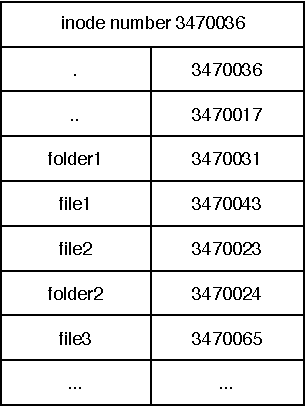
\includegraphics[width=0.3\linewidth]{./images/inode_catalog.pdf}
  \end{tabular}
\end{table}

Имя файла сопоставлено с номером inode, имя директории -- с номером inode. Именно обычные файлы и директории долговременно хранятся во вторичной памяти.

Невозможно не хранить имена директорий в долговременной памяти, так как иначе к ним не будет доступа (выключили комп, все имена исчезли и остались одни номера inode).

\subsection{struct file}

Существует 2 типа файлов --- файл, к-ый лежит на диске и открытый файл. Открытый файл -- файл, который открывает процесс

\textbf{Кратко}

struct file описывает открытый файл.

\textbf{Подробно}

Если файл просто лежит на диске, то через дерево каталогов можно увидеть это. 

Увидеть можно только подмонтированную ФС.

А есть открытые файлы --- файлы, с которыми работают процессы.

Открыть файл может только процесс. Если файл открывается потоком, то он в итоге все равно открывается процессом (как ресурс). Ресурсами владеет процесс.


\subsubsection{Таблицы открытых файлов}

Помимо таблицы открытых файлов процесса (есть у каждого процесса), в системе есть одна таблица на все открытые файлы (на которую ссылаются таблицы процессов).

Причем в этой таблице на один и тот же файл (с одним и тем же inode) мб создано большое кол-во дескрипторов открытых файлов, т.к. один и тот же файл мб открыт много раз. 

Каждое открытие файла с одним и тем же inode приведет к созданию дескриптора открытого файла.

При открытии файла его дескриптор добавляется:
\begin{enumerate}
    \item в таблицу открытых файлов процесса (struct file\_struct)
    \item в системную таблицу открытых файлов
\end{enumerate}

Каждый дескриптор struct file имеет поле f\_pos. При работе с файлами это надо учитывать.

Один и тот же файл, открытый много раз без соотв. способов взаимоискл. будет атакован, что приведет к потере данных.

\sout{Гонки при разделении файлов -- один и тот же файл мб открыт разными процессами.}

\subsubsection{Определение struct file}
\begin{lstlisting}
    struct file {
  struct path    f_path;
  struct inode    *f_inode;  /* cached value */
  const struct file_operations  *f_op;
        ...
  atomic_long_t    f_count;// кол-во жестких ссылок
  unsigned int     f_flags;
  fmode_t      f_mode;
  struct mutex    f_pos_lock;
  loff_t      f_pos;
  ...
  struct address_space  *f_mapping;
  ...
};
\end{lstlisting}
Как осуществляется отображение файла на физ. страницы? - дескриптор открытого файла имеет указатель на inode (файл на диске).

\textbf{Связь между struct file и struct file operations}

Файл должен быть открыт. Соответственно для открытого файла должен быть создан дескриптор. В этом дескрипторе имеется указатель на struct file\_operations. Это либо стандартные (установленные по умолчанию) операции на файлах для конкретной файловой системы, либо зарегистрированные разработчиком (собственные функции работы с файлами собственной файловой системы).

\begin{lstlisting}
	struct file_operations {
	struct module *owner;
	loff_t (*llseek) (struct file *, loff_t, int);
	ssize_t (*read) (struct file *, char __user *, size_t, loff_t *);
	ssize_t (*write) (struct file *, const char __user *, size_t, loff_t *);
	...
	int (*open) (struct inode *, struct file *);
	...
	int (*release) (struct inode *, struct file *);
	...
} __randomize_layout;
\end{lstlisting}

Разработчики драйверов должны регистрировать свои функции read/write. В UNIX/Linux все файл как раз для того, чтобы свести се действия к однотипным операциям read/write и не размножать их, а свести к большому набору операций.

Для регистрации своих функций используется(-лась) struct file\_operations. С некоторой версии ядра 5.16+ (примерно) появилась struct proc\_ops. В загружаемых модулях ядра можно использовать условную компиляцию:

\begin{lstlisting}
#if LINUX_VERSION_CODE >= KERNEL_VERSION(5,6,0)
#define HAVE_PROC_OPS
#endif

#ifdef HAVE_PROC_OPS
static struct proc_ops fops = {
    .proc_read = fortune_read,
    .proc_write = fortune_write,
    .proc_open = fortune_open,
    .proc_release = fortune_release,
};
#else
static struct file_operations fops = {
    .owner = THIS_MODULE,
    .read = fortune_read,
    .write = fortune_write,
    .open = fortune_open,
    .release = fortune_release,
};
#endif
\end{lstlisting}

proc\_open и open имеют одни и те же формальные параметры (указатели на struct inode, struct file). С другими функциями аналогично.

Зачем так сделано? --- proc\_ops сделана для того, чтобы не вешаться на file\_operations, которые используются драйверами. Функции file\_operations настолько важны для системы, что их решили освободить от работы с ФС proc.

\section{Адресация файлов большого размера в файловой системе extX}

\begin{table}[h!]
  \centering
  \begin{tabular}{p{1\linewidth}}
    \centering
    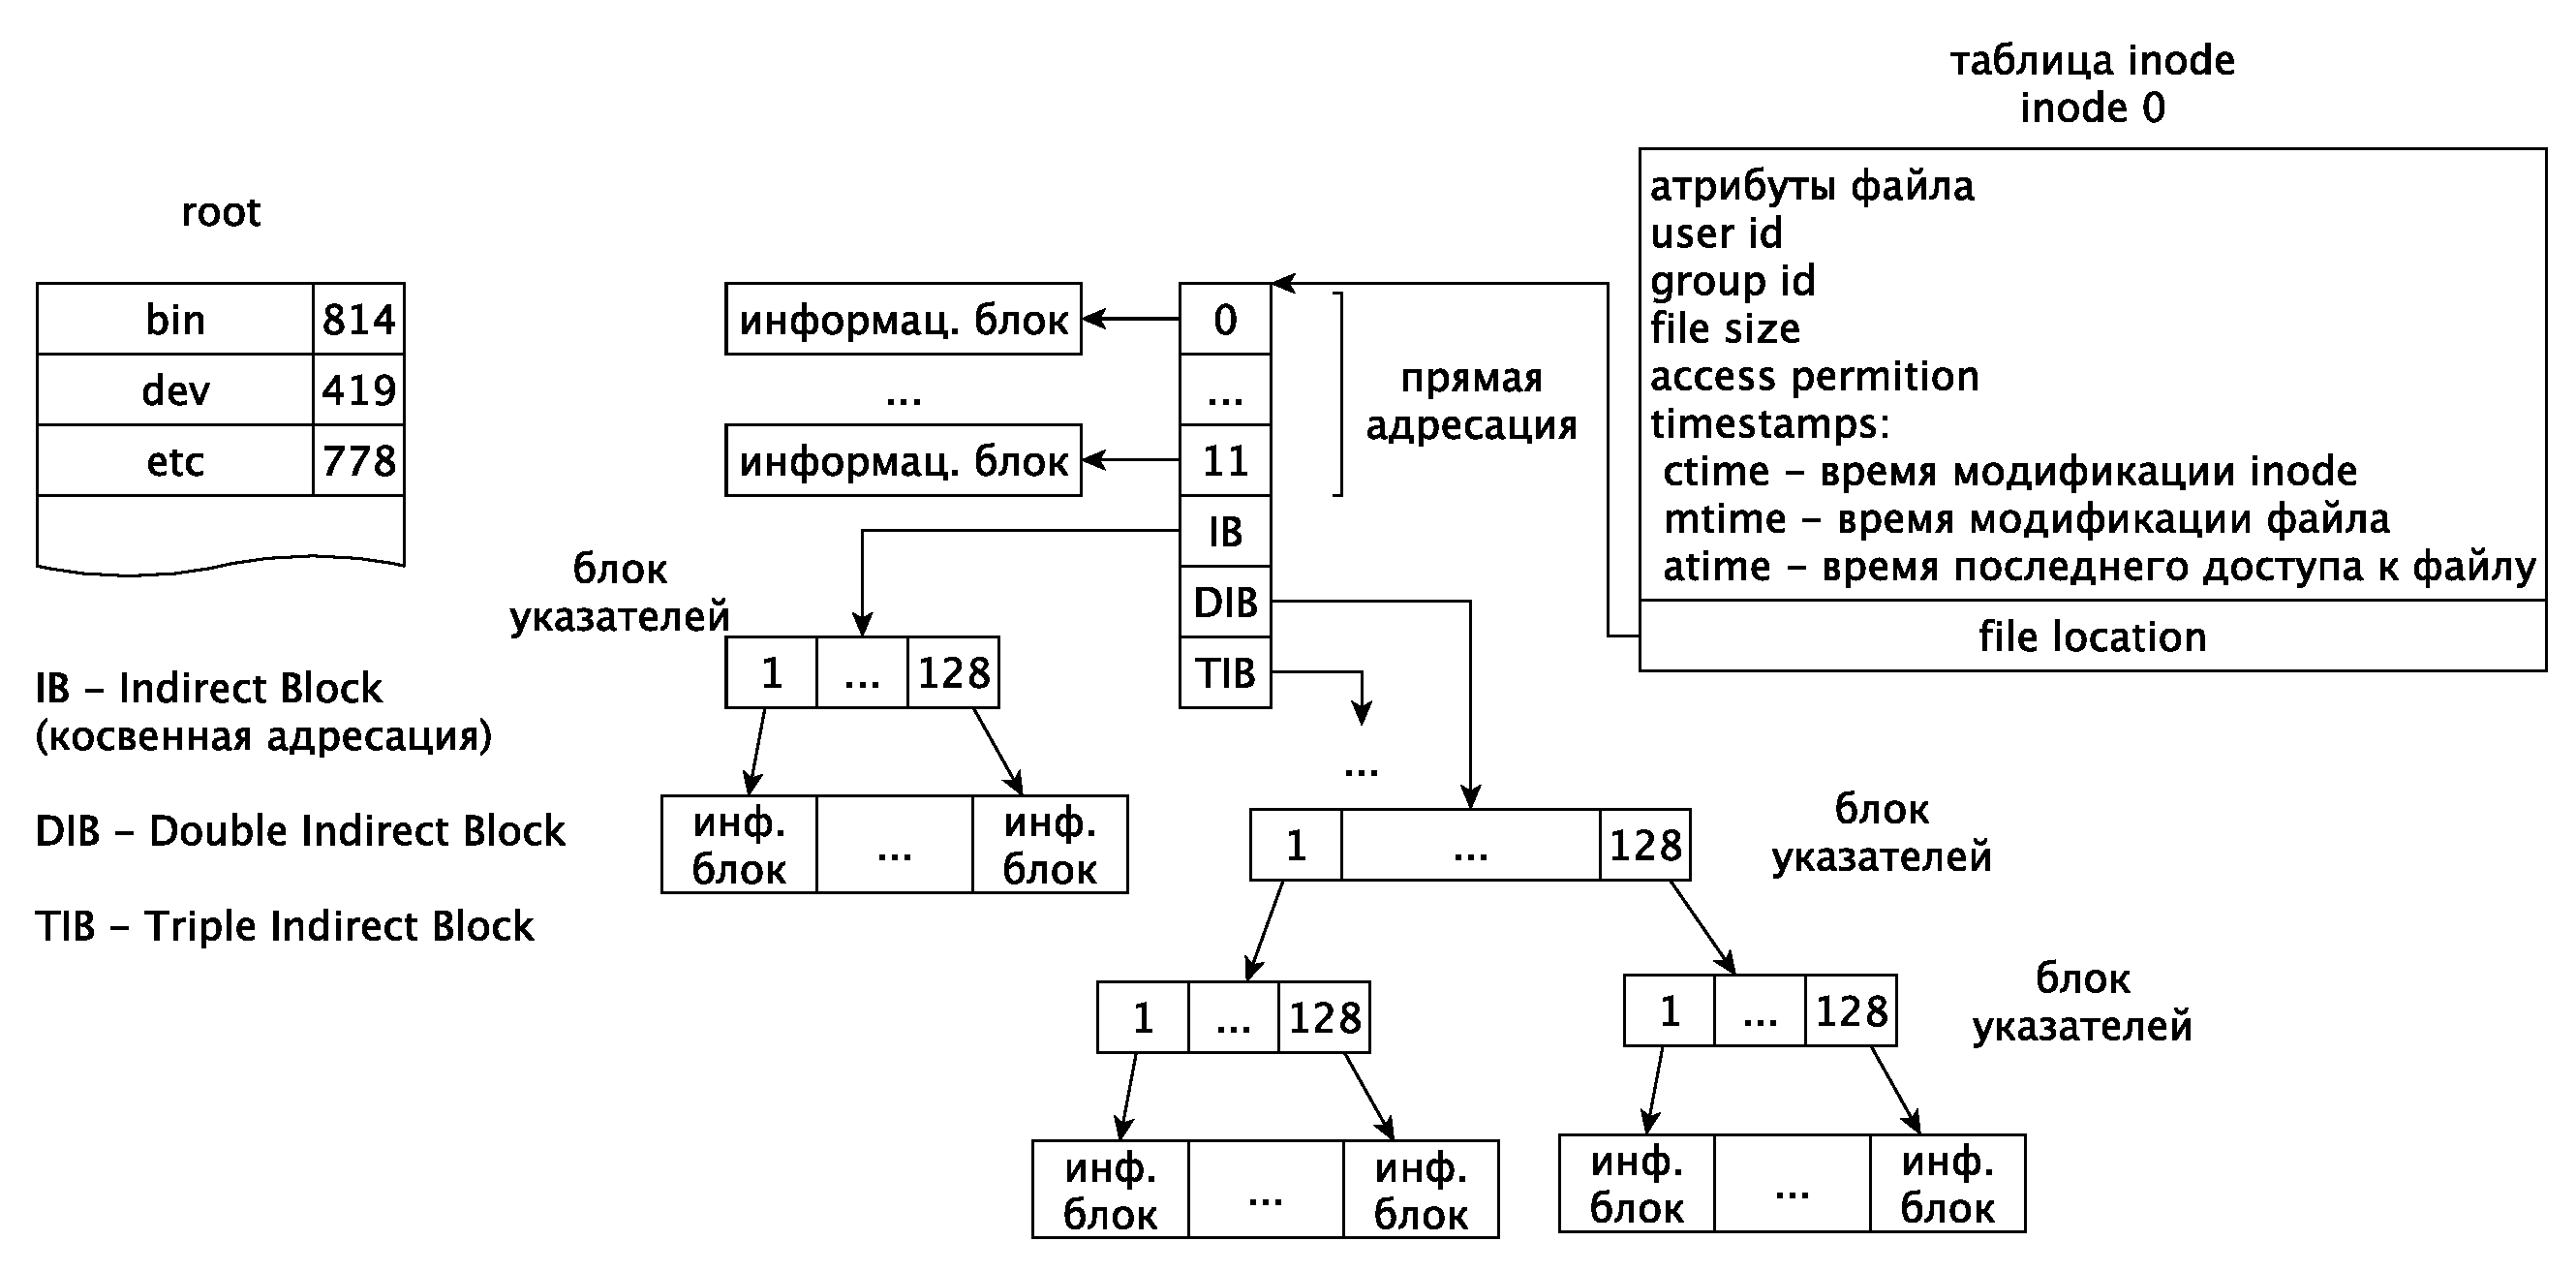
\includegraphics[width=0.8\linewidth]{./images/extX.pdf}
  \end{tabular}
\end{table}

Чтобы иметь возможность хранить файлы очень большого размера, еще в 80-х была предложена схема с прямой и косвенной адресацией, двойной и тройной косвенной адресацией. Каждый адрес хранит адрес конкретного блока физического диска, в котором хранится информация, записанная в файл.

Прямая адресация --- быстрый доступ к блоку. Время доступа --- плата за возможность адресации больших файлов.

\section{Пример, показывающий доступ к файлу /usr/ast/mbox}

\begin{table}[h!]
  \centering
  \begin{tabular}{p{1\linewidth}}
    \centering
    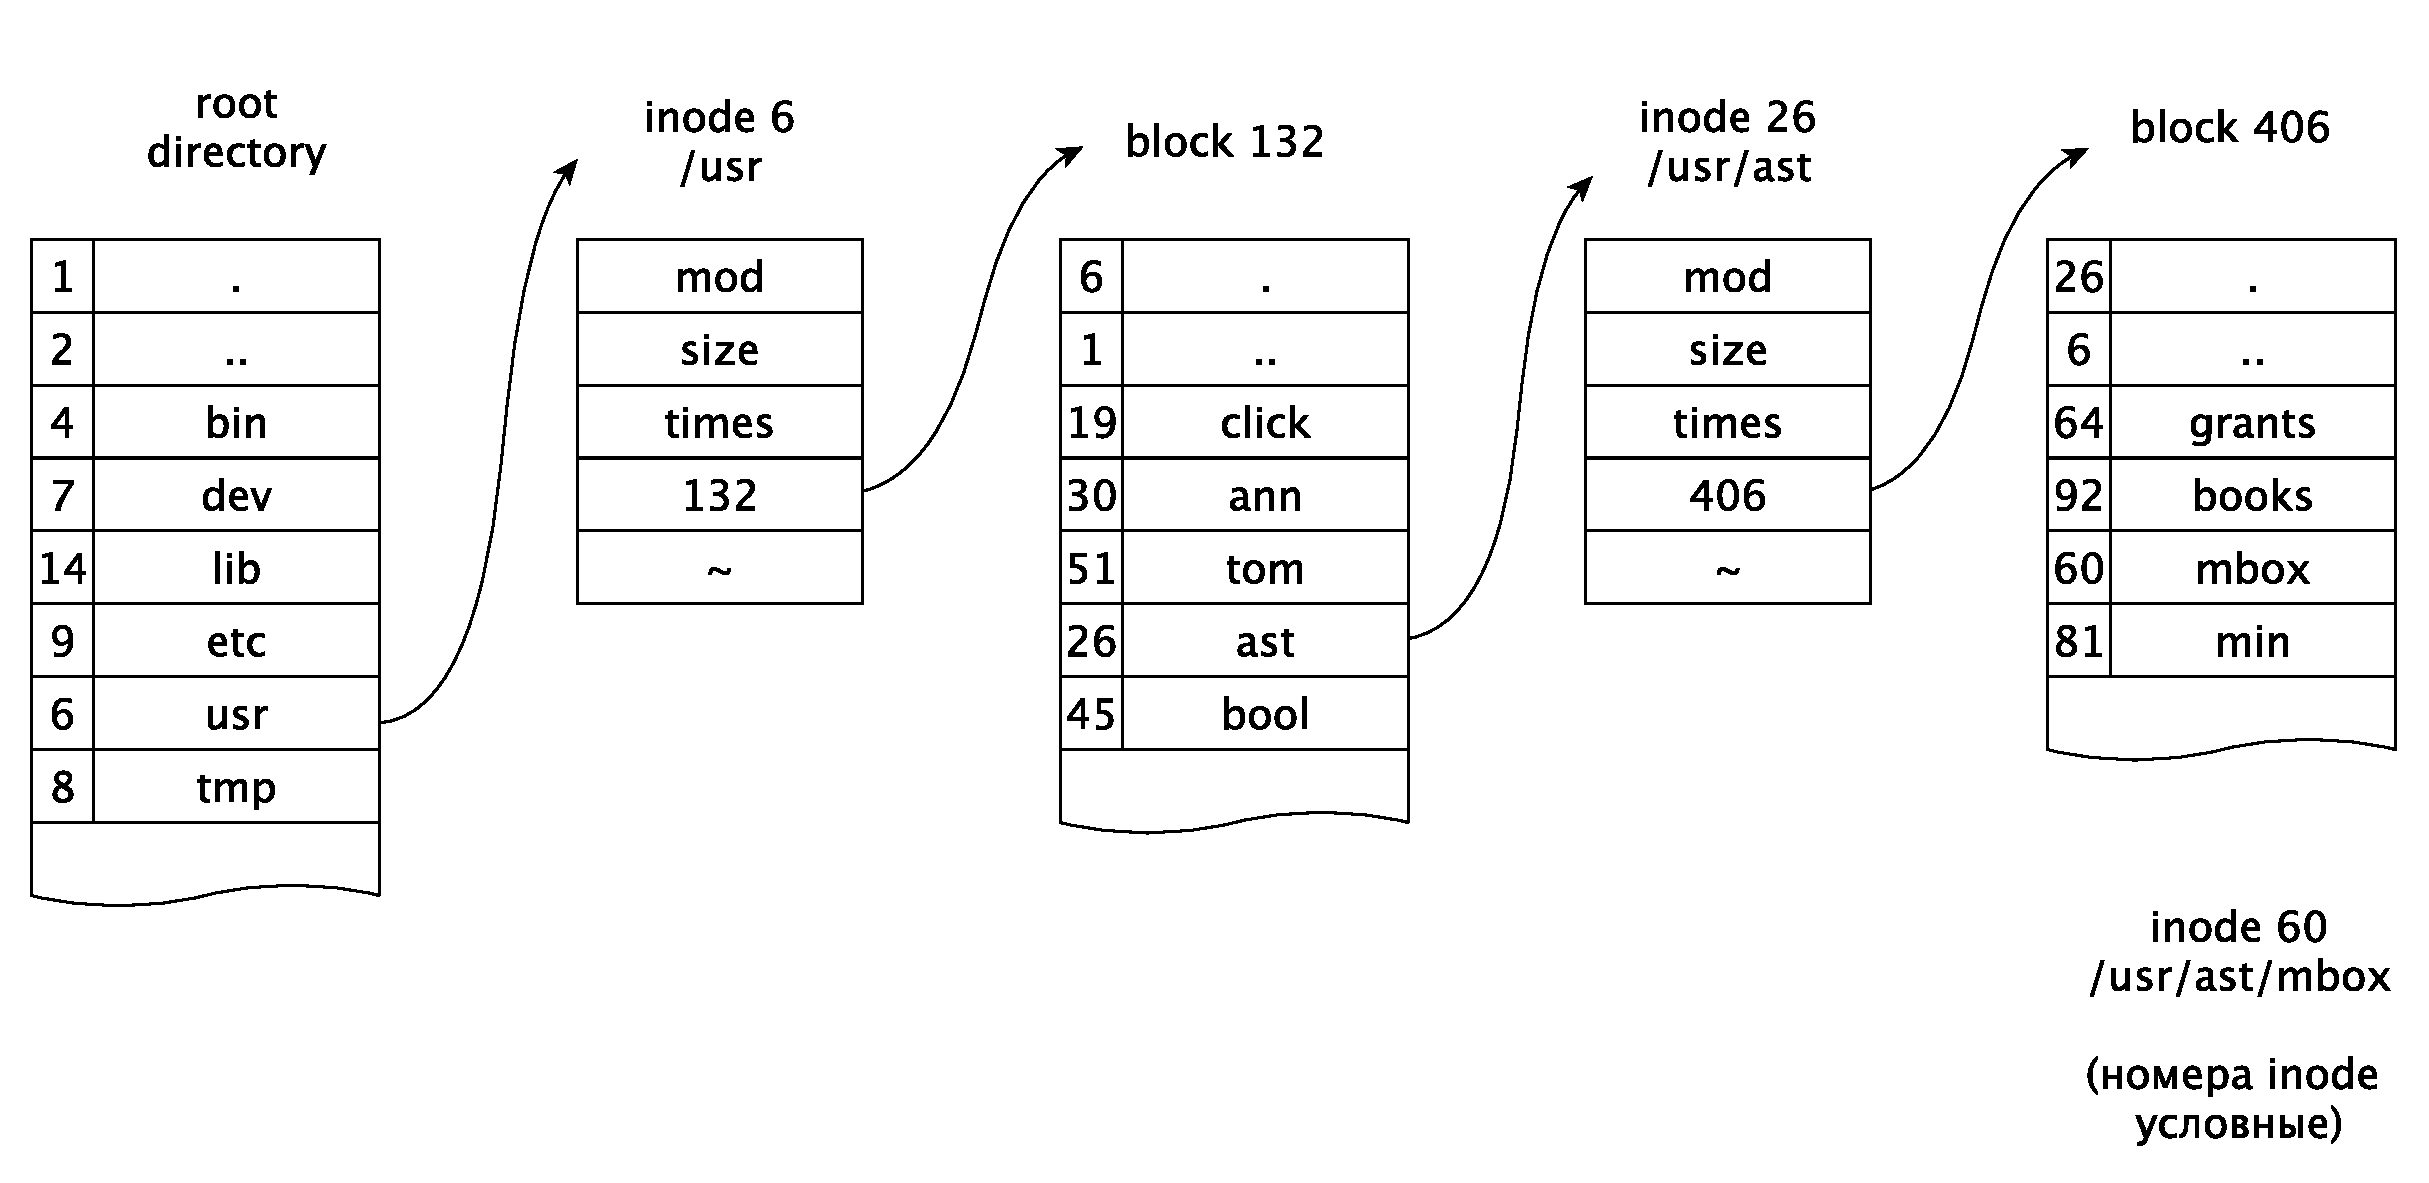
\includegraphics[width=0.8\linewidth]{./images/mbox.pdf}
  \end{tabular}
\end{table}

В дисковом inode хранятся адреса блоков, в которых находится информация, записанная в соответствующий файл. struct inode содержит поля mod, size, times, ..., которые определяют время последнего обращения, модификации и номер блока (адрес блока). inode данной директории (/usr) содержит номер блока, в котором находится информация директории /usr. Из содержимого блока получаем номер inode /usr/ast --- 26. Получаем номер inode /usr/ast/mbox --- 60. далее произойдет обращение к соответствующей информации. Всего 3 элемента пути, и столько обращений к внешней памяти. Поэтому все нужно кешировать.

\section{Монтирование файловых систем}

Фактически VFS — интерфейс, с помощью которого ОС может работать с большим количеством файловых систем.

Основной такой работы (базовым действием) является монтирование: прежде чем файловая система станет доступна (мы сможем увидеть ее каталоги и файлы) она должна быть смонтирована.

Монтирование — подготовка раздела диска к использованию файловой системы. Для этого в начале раздела диска выделяется структура super\_block, одним из полей которой является список inode, с помощью которого можно получить доступ к любому файлу файловой системы.

Когда файловая система монтируется, заполняются поля struct vfsmount, которая представляет конкретный экземпляр файловой системы, или, иными словами, точку монтирования. Точкой монтирования является директория дерева каталогов.

Вся файловая система должна занимать либо диск, либо раздел диска и начинаться с корневого каталога.

Любая файловая система монтируется к общему дереву каталогов (монтируется в поддиректорию).

И эта подмонтированная файловая система описывается суперблоком и должна занимать некоторый раздел жесткого диска ("это делается в процессе монтирования").

Когда файловая система монтируется, заполняются поля структуры super\_block.

super\_block содержит информацию, необходимую для монтирования и управления файловой системой.

\begin{quote}
Пример: мы хотим посмотреть содержимое флешки. Флешка имеет свою файловую систему, она может быть подмонтирована к дереву каталогов, и ее директории, поддиректории и файлы, которые мы сохраним на флешке, будут доступны. Потом мы достаем флешку. "Хорошая" система контролирует это и сделает демонтирование файловой системы за нас.
\end{quote}

\begin{quote}
Если в системе присутствует некоторый образ диска image, а также создан каталог, который будет являться точкой монтирования файловой системы dir, то подмонтировать файловую систему можно, используя команду: mount -o loop -t myfs ./image ./dir

Параметр -o указывает список параметров, разделенных запятыми. Одним из прогрессивных типов монтирования, является монтирование через петлевое (loop, по сути, это «псевдоустройство» (то есть устройство, которое физически не существует --- виртуальное блочное устройство), которое позволяет обрабатывать файл как блочное устройство) устройство. Если петлевое устройство явно не указано в строке (а как раз параметр -o loop это задает), тогда mount попытается найти неиспользуемое в настоящий момент петлевое устройство и применить его.

Аргумент следующий за -t указывает тип файловой системы.

./image - это устройство. ./dir - это каталог.

umount — команда для размонтирования файловой системы:

umount ./dir
\end{quote}

\section{Команда mount и функции монтирования}

Любая файловая система может быть подмонтирована много раз. Для этого ядро предоставляет функцию mount.

В ядре определено несколько функций mount.
\begin{lstlisting}
typedef int (*fill_super_t)(struct super_block *, void *, int);
struct dentry *mount_bdev(struct file_system_type *fs_type, int flags, const char *dev_name, void *data, fill_super_t fill_super);
struct dentry *mount_nodev(struct file_system_type *fs_type, int flags, void *data, fill_super_t fill_super);
struct dentry *mount_single(struct file_system_type *fs_type, int flags, void *data, fill_super_t fill_super);
\end{lstlisting}

\begin{itemize}
    \item mount\_bdev — для монтирования ФС, находящейся на блочном устройстве,
    \item mount\_nodev — для монтирования ФС, не связанной ни с каким устройством,
    \item mount\_single — для монтирования ФС, точки монтирования которой разделяют один единственный экземпляр ФС.
\end{itemize}

И в mount\_bdev(), и в mount\_nodev() вызывается функция fill\_super(), которая выполняет основные действия по инициализации struct super\_block.

Эти функции возвращают объект dentry, и этим объектом должен быть root. Для файловой системы необходимо создать root. Это позволит выполнить монтирование файловой системы. Для root надо создать inode.

\textbf{Пример из лабораторной VFS:}

\begin{lstlisting}
#include <linux/module.h>
#include <linux/kernel.h>
#include <linux/init.h>
#include <linux/init_task.h>
#include <linux/fs.h>
#include <linux/slab.h>
#include <linux/time.h>

MODULE_LICENSE("GPL");
MODULE_AUTHOR("Ekaterina Karpova");

#define MAGIC_NUM 0x12528391

#define CACHE_SIZE 1024
#define CACHE_NAME "kittyfs_cache"
static struct kmem_cache *cache = NULL;
static struct kittyfs_inode **inode_cache = NULL;
static size_t cache_index = 0;

static struct kittyfs_inode
{
    int i_mode;
    unsigned long i_ino;
} kittyfs_inode;

static void kittyfs_kill_sb(struct super_block *sb){
    printk(KERN_INFO "+ kittyfs: kill super block");
    kill_anon_super(sb);
}

static void kittyfs_put_sb(struct super_block *sb)
{
    printk(KERN_INFO "+ kittyfs: superblock destroy called");
}

static struct super_operations const kittyfs_sb_ops = {
    .put_super = kittyfs_put_sb,
    .statfs = simple_statfs,
    .drop_inode = generic_delete_inode,
};

static struct inode *kittyfs_new_inode(struct super_block *sb, int ino, int mode)
{
	struct inode *res;
	res = new_inode(sb);
	if (!res)
		return NULL;
	res->i_ino = ino;
    res->i_mode = mode;
    res->i_atime = res->i_mtime = res->i_ctime = current_time(res);
    res->i_op = &simple_dir_inode_operations;
    res->i_fop = &simple_dir_operations;
    res->i_private = &kittyfs_inode;
    
    if (cache_index >= CACHE_SIZE)
    {
    	return NULL;
    }
    
    inode_cache[cache_index] = kmem_cache_alloc(cache, GFP_KERNEL);
    if (inode_cache[cache_index])
    {
    	inode_cache[cache_index]->i_ino = res->i_ino;
    	inode_cache[cache_index]->i_mode = res->i_mode;
    	cache_index++;
    }
    return res;
}

static int kittyfs_fill_sb(struct super_block *sb, void *data, int silent)
{
    struct dentry *root_dentry;
    struct inode *root_inode;
    sb->s_blocksize = PAGE_SIZE;       
    sb->s_blocksize_bits = PAGE_SHIFT;
    sb->s_magic = MAGIC_NUM;
    sb->s_op = &kittyfs_sb_ops;
    root_inode = kittyfs_new_inode(sb, 1, S_IFDIR | 0755);
    if (!root_inode)
    {
        printk(KERN_INFO "+ kittyfs: cannot make root inode");
        return -ENOMEM;
    }
    root_dentry = d_make_root(root_inode);
    if (!root_dentry)
    {
        printk(KERN_ERR "+ kittyfs: cannot make root dentry");
        return -ENOMEM;
    }
    sb->s_root = root_dentry;
    return 0;
}

static struct dentry *kittyfs_mount(struct file_system_type *type, int flags, const char *dev, void *data)
{
    struct dentry *const root_dentry = mount_nodev(type, flags, data, kittyfs_fill_sb);
    if (IS_ERR(root_dentry))
        printk(KERN_ERR "+ kittyfs: cannot mount");
    else
        printk(KERN_INFO "+ kittyfs: mount successful");
    return root_dentry;
}

static void kittyfs_slab_constructor(void *addr)
{
    memset(addr, 0, sizeof(struct kittyfs_inode));
}

static struct file_system_type kittyfs_type = {
    .owner = THIS_MODULE,
    .name = "kittyfs",
    .mount = kittyfs_mount,
    .kill_sb = kittyfs_kill_sb,
};

static int __init kittyfs_init(void)
{
    int err = register_filesystem(&kittyfs_type);

    if (err != 0){
        printk(KERN_ERR "+ kittyfs: cannot register filesystem");
        return err;
    }

    if ((inode_cache = kmalloc(sizeof(struct kittyfs_inode*)*CACHE_SIZE, GFP_KERNEL)) == NULL)
    {
        printk(KERN_ERR "+ kittyfs: Can't kmalloc.\n");
        return -ENOMEM;
    }

    if ((cache = kmem_cache_create(CACHE_NAME, sizeof(struct kittyfs_inode), 0, SLAB_HWCACHE_ALIGN, kittyfs_slab_constructor)) == NULL)
    {
        printk(KERN_ERR "+ kittyfs: cannot create cache");
        kmem_cache_destroy(cache);
        kfree(inode_cache); 
        return -ENOMEM;
    }

    printk(KERN_INFO "+ kittyfs: module loaded");
    return 0;
}

static void __exit kittyfs_exit(void)
{
    int err;
    int i;
    
    for (i = 0; i < cache_index; i++)
    	kmem_cache_free(cache, inode_cache[i]);
    
    kmem_cache_destroy(cache);
    kfree(inode_cache);

    err = unregister_filesystem(&kittyfs_type);
    if (err != 0)
        printk(KERN_ERR "+ kittyfs: cannot unregister filesystem");
    else
        printk(KERN_INFO "+ kittyfs: module is unloaded");
}

module_init(kittyfs_init);
module_exit(kittyfs_exit);
\end{lstlisting}






